% !TeX root = CH04-WaterBalanceModel.tex
% !TeX spellcheck = en_US
% !TeX encoding = UTF-8
\renewcommand{\thechapter}{4}
\chapter{Evaluation of NPS Return Flow to the River Using a Water Balance Model}
\label{chap:WaterBalanceModel}

\begin{linenumbers}
\section{Water Balance Model Applied to the LARV}
\label{sec:AppliedWaterModel}

The purpose of the water balance model is to determine the volume of unaccounted for water in each reach.  We begin with a basic water balance model as describe in most hydrology texts --- \parencite{wanielista1997}.
\begin{equation}
	\textnormal{change in storage = inputs - outputs} \nonumber
\end{equation}

Adding the variables, both known and unknown, present in the LARV we have the following equation:
\begin{equation}
\label{eq:water1}
	\frac{\Delta S}{\Delta t} = Q_{in,US} + \sum Q_{in} + P + R + B - Q_{out,DS} - \sum Q_{out} - E - T - F + X
\end{equation}
\begin{longtable}{r p{5.5in}}
	Where: \\
	$\displaystyle \frac{\Delta S}{\Delta t}$ =&Stored volume change between time steps.\\
	$ Q_{in,US} $ = & Flow in the river entering the study reach at the upstream end.\\
	$ \displaystyle \sum Q_{in} $ = & Flow gained by the river from tributaries and other gauged sources.\\
	$ P $ = & Volume of water gained to the river due to precipitation falling directly on the river's surface.\\
	$ R $ = & Volume of water gained to the river due to precipitation runoff from adjacent land. \\
	$ B $ = & Volume of water gained to the river due to subsurface flow. \\
	$ Q_{out,DS} $ = & Flow in the river leaving the study reach at the downstream end.\\
	$ \displaystyle \sum Q_{out} $ & Flow lost from the river to canals and other gauged sinks.\\
	$ E $ = & Volume of water lost from the river due to direct evaporation from the water's surface.\\
	$ T $ = & Volume of water lost from the river due to plant transpiration.\\
	$ F $ = & Volume of water lost from the river due to infiltration into the subsurface flow.\\
	$ X $ = & Water volume gains and losses to/from unknown sources and sinks.\\
\end{longtable}

The inclusion of the $ X $ term signifies one of two types of unknown values addressed in this thesis.  There are known unknowns, which are directly addressed and unknown unknowns.  Known unknowns are those values or terms which are known to exist, but the magnitude and sign of their effect is unknown and/or immeasurable.  Unknown  unknowns are those values or terms which we do not know exist.  Their existence and effect on a system are yet to be discovered.  We assume with the current state of chemistry and physics, that the $ X $ term is insignificant.  However, we cannot discount it from our analysis.

If we combine the terms that are unknown or unmeasured, we arrive at the following equation:
\begin{equation}
	\label{eq:water01}
	\frac{\Delta S}{\Delta t} = Q_{in,US} + \sum Q_{in} + P - Q_{out,DS} - \sum Q_{out} - E + Q_{UNPS}
\end{equation}
\begin{tabular}{r p{5.5in}}
	Where: \\
	\Qnps = & The sum of gains from non-point sources and losses to non-point sinks \\
		= &$ Q_{UNPS} = R + B - T - F + Q_{U,in} - Q_{U,out} +X $.\\ 
\end{tabular}\\

%\emph{III - define $Q_U$ constituents}\\
There is no reasonable method for differentiating the components of \Qnps, therefore the abbreviation NPS in this thesis refers to both non-point sources and non-point sinks.   \Qnps includes the non-point source gains from groundwater sources($ B $), non-point source losses to groundwater sinks {}$ F $), transpiration losses from plants in the river channel ($ T $), and gains from precipitation runoff from adjacent land ($ R $).  Additionally, this term includes ungauged flows leaving and entering the river.  Ungauged gains to the river ($ Q_{U,in} $) are suspected to be primarily in the form of irrigation drainage from adjacent farmland.  Other sources could be due to errors in underestimating flows entering the river or overestimating flows leaving the river.  Ungauged losses from the river ($ Q_{U,out} $) are suspected to be primarily in the form of minor or unauthorized withdrawals from the river channel.  Of the ungauged flows, irrigation drainage from adjacent farmlands is assumed to be the largest contributor.

The two groundwater components of \Qnps are suspected of being the largest components of \Qnps.  Water transfer between the aquifer and river happens continually whereas $ Q_{U,in} $, $ Q_{U,out} $, $ R $, and $ T $ are not continuous.  $ Q_{U,in} $ and $ Q_{U,out} $ only occur periodically when individuals actively withdraw from the river or allow irrigation runoff to return to the river.  $ R $ only occurs during rain events.  Within the LARV, most rainwater is captured in irrigation canals.  Only precipitation falling in the riparian zone is likely to reach the river.  $ T $ only occurs during growing season.  This value is also only considering the transpiration happening within the river channel and does not include the riparian zone.  Any losses due to transpiration in the riparian zone are first considered river losses to the aquifer ($ F $).

Re-arranging equation \eqref{eq:water01} to solve for the unknown values produces equation \ref{water02}.  Due to the nearly identical method of calculating flow ($ Q $) and it's associated error and uncertainty, these terms were associated with each other.  Likewise, the precipitation ($ P $) and evaporation ($ E $) terms were associated with each other.
\begin{equation}
	\label{eq:water2}
	Q_{UNPS} = \left( Q_{out,DS} + \sum Q_{out} - Q_{in,US} - \sum Q_{in} \right) + \frac{\Delta S}{\Delta t} - \left( P + E \right)\\ 
\end{equation}

This model is further simplified to Equation \ref{eq:water3} which combines terms that are calculated using similar methods to facilitate discussion.
\begin{equation}
	\label{eq:water3}
	Q_{UNPS} = \frac{\Delta S}{\Delta t} - \sum Q_{Surface} - \sum Q_{Atm}\\ 
\end{equation}
\begin{tabular}{r p{5.5in}}
	Where:&\\
	$ \displaystyle \frac{\Delta S}{\Delta t} $ = & Reach storage change per time-step.\\
	$ \displaystyle \sum Q_{Surface} $ = & Sum of flows added and removed from the reach per time-step. \\
		= & $ Q_{in,DS} + \sum Q_{in} - Q_{out,US} - \sum Q_{out} $\\
	$ Q_{Atm} $ = & The sum of precipitation gains and evaporation losses, per time step.\\
		= & $ P - E $\\
\end{tabular}\\

A time step of one day was established for all models calculated in this thesis.  Most of the data from agencies is readily available in average daily format.  While most of the data could also be obtained in hourly or quarter-hourly format, it was assumed that the additional information would not improve model accuracy.

\clearpage{}
\section{Stochastic and Deterministic Models}
\label{sec:StochAndDetermModels}

Deterministic and stochastic models are used in both the unaccounted for water and mass balance models.  Deterministic models are fully determined by the input parameters or variables.  Randomness of any kind is not included.  Stochastic models extend deterministic models by including one or more random parameters.  Given the same input parameter values, a stochastic model will produce different results with each iteration.

There are many recognized methods for solving stochastic models.  Solutions to these models are not definite and the term "solve" must be taken loosely.  Any individual solution from a stochastic model is one of a potentially infinite number of possible solutions.  The Monte Carlo (MC) simulation technique was used to obtain solutions for all stochastic models in this thesis.  The MC technique is conceptually simple.  The stochastic model is repetitively solved in a series of iterations.  The combined solutions from all iterations are used to define the solution statistics of the model.  

The number of iterations performed is determined by calculating and analyzing a set of identifier statistic(s) after each run.  Identifier statistic(s) are those that the modeler has determined to be of value in determining when to terminate the model.  These statistics are monitored to identify when the change in the statistic has reached a predetermined threshold.  It was determined that for the sake of simplicity, all of the models calculated in this thesis would use the same number of iterations.  The USR mass balance model is the most complex model as it has the largest number of input variables and uncertainty terms.  The identifier statistics used were the mean, variance, and skewness which are the first, second, and third moments of the probability density.  These were calculated for each iteration.  The threshold between the observed iteration and the previous iteration was fixed at 0.1\%.  The identifier statistics reached the threshold in the following order: mean, variance, and skewness.  Skewness reached its break point shortly before the 500th iteration.  A judgment call was made to increase the factor of safety.  Therefore, the number of stochastic model iterations was fixed at 5,000.  The fourth moment, kurtosis, was also calculated and analyzed for each iteration.  It was found to be too sensitive as it did not consistently stay within the accepted cutoff threshold of 0.1\%.  It is assumed that this sensitivity is due to the existence of a significant number of outliers that cause the distribution of results to be non-normal.

\section{Error and Uncertainty.}
\label{sec:ErrorAndUncertainty}

Any problem that measures variable natural processes must account for parameter and model uncertainties \parencite{vicens1975}.  Parameter uncertainty is derived from measurement error, spatial variability, and temporal variability \parencite{herschy2002}.  Measurement error is the difference between the true and measured values.  Most of this error type is due to instrument measurement inaccuracies due to either error inherent in the instrument or from errors in calibration or measurement.  Measurement errors inherent to the instrument are uncorrectable and cannot be accounted for within the model.  Errors due to calibration or measurement deviations are only correctable at the time of measurement or calibration and cannot be accounted for within the model.

Spatial variability is the difference in the true value at different points when measured at the same time.  Data collected at a single given point in space may not be representative of the area it is assumed to represent due to spatial variability.  This can manifest itself even with very small distances between measurements.  Temporal variability is the difference in the true value at the same point, but at different times.  Data collected at a one time may not be representative of the time frame it is assumed to represent due to temporal variability \parencite{Gates1996}.  Again, this can be manifested even over small time differences.  Due to instrument error, the spatiotemporal variability of the measured object, and the inability to know the true value of the measurement, reported parameter values should be treated as random variables \parencite{haan1989,haan2002}.

Almost all of the data was obtained from outside agencies and was not collected by the research team.  These agencies have data uncertainty ranges that account for all parameter uncertainties.  These uncertainties are expressed in accordance with the ISO Guide to Expression of Uncertainty in Measurement (GUM) \parencite{gum2008}.  While the GUM classifies uncertainty as either "Type A" or "Type B", the all of the data included in this thesis has uncertainty evaluations described as "Type B".  Type B evaluations usually use standard deviations and assumed probability distributions obtained from scientific judgment, available information, and possible variability of a measurement.

The data originators have provided uncertainty ranges which include instrument measurement random error and uncertainties due to temporal variations of the measured location.  The root mean square method is used to estimate the uncertainty related to measurement of water quantity and water quality values \parencite{harmel2007, gum2008}.  \textcite{harmel2007} describe this measurement uncertainty as the “probably error range”, and quantify upper and lower uncertainty boundaries for measured data points as the following when attempting to specify an expected range of expected values.
\begin{align}
	\sigma^2 = \left( \frac{O_i-UO_{i}(l)}{3.9} \right)^2  &  \phantom{xxxxxxxx} or  & 	\sigma^2 = \left( \frac{UO_{i}(u)-O_i}{3.9} \right)^2 \label{eq:uncertainty1}
\end{align}
\begin{tabular}{r p{5.5in}}
	Where:\\
	$ \sigma^2 $ = & variance about measured data value $ O_i $.\\
	$ O_i $ = & measured value.\\
	$ UO_i $ = & upper $ (u) $ and lower $ (l) $ uncertainty boundaries.\\
	$ 3.9 $ = & number of standard deviations accounting for $ >99.99 $\% of a normal probability distribution
\end{tabular}\\

The data collected for this thesis is assumed to represent the mean of a normal distribution of possible values.  The upper and lower bounds of the distributions are given as either a percent or value deviation from the mean.  Equation \ref{eq:uncertainty1} is re-written from the definition found in \textcite{harmel2007} to that found in equation \ref{eq:uncertainty2}.
\begin{align}
	\sigma^2 = \left( \frac{\mu - (\mu - \mu p)}{3.9} \right)^2  &  \phantom{wordsssssss} or \phantom{s}  & 	\sigma^2 = \left( \frac{(\mu + \mu p) - \mu}{3.9} \right)^2 \label{eq:uncertainty2}
\end{align}

\begin{tabular}{r p{5.5in}}
	Where:\\
	$ \mu $ = & the reported value (assumed to be the mean).\\
	$ p $ = & the reported percent deviation from $ \mu $.\\
\end{tabular}\\

Both of these equations in \ref{eq:uncertainty2} simplify to equation \ref{eq:uncertainty3}.  The standard deviation is shown as the calculated result due to the requirements of the modeling software.
\begin{equation}
\sigma = \frac{\mu p}{3.9}
\label{eq:uncertainty3}
\end{equation}

When the upper and lower bounds are defined as a fixed value deviation from the reported value, then equation \ref{eq:uncertainty1} becomes:

\begin{align}
	\sigma^2 = \left( \frac{\mu - (\mu - v)}{3.9} \right)^2  &  \phantom{wordsssssss} or \phantom{s}  & 	\sigma^2 = \left( \frac{(\mu + v) - \mu}{3.9} \right)^2 \label{eq:uncertainty4}
\end{align}
\begin{tabular}{r p{5.5in}}
	Where:\\
	$ v $ = & the reported value deviation from $ \mu $.\\
\end{tabular}\\

In this case, both equations in \ref{eq:uncertainty4} simplify to:
\begin{equation}
\sigma = \frac{v}{3.9}
\label{eq:uncertainty5}
\end{equation}

The difference between a model's calculated or estimated value and the reported value is called a residual.  The distribution of residuals is the model uncertainty.  These distributions are uni-variate and do not have predefined shapes.  There are a variety of statistical and graphical tools available to analyze unknown residual distributions to determine a best fit parametric distribution.  The two graphical tools used in this thesis to analyze distributions are the histogram and the kernel density estimate.

Non-parametric distribution models are used as an aid for analyzing uni-variate data sets.  Specifically, kernel density estimates (KDE) are used in conjunction with histograms to assist in visual analysis of the data.  Figure \ref{fig:ExampleDistAnalysis} is an example of a random sample of one of the input data sets used in this thesis.  The curve is the KDE.  The short vertical lines between the histogram and the x-axis, called a rug, depict the data values.  This figure adequately displays the resulting differences between histograms and KDE.  KDEs can more accurately depict data groupings that are lost in histogram bins.  The histogram leads us to believe that the data has a strong tendency to be near zero, wile the KDE shows that the majority of the data is between 0-20.  Histograms can more accurately depict extremes or cut-off values.  In the figure, there are no values less than zero.  The histogram clearly shows this while the KDE shows that there are values less than zero.  Both histograms and KDE are used throughout this thesis to assist in the description of distributions.  A rug is also presented with the histogram whenever the quantity of data allows for adequate data presentation.  A rug is not included when the data set is too large to allow for discreet identification of data values.

\begin{figure}[htbp]
\centering
	\includegraphics[width=6in]{"Figures/Example KDE"}
	\caption[Example kernel density estimate.]{Example kernel density estimate.  The data is a random sample of an input variable used in this thesis.  The curve depicts the kernel density estimate.  The short vertical lines between the histogram and the x-axis, called a rug, depict the data values.}
	\label{fig:ExampleDistAnalysis}
\end{figure}

Determining which parametric distribution best fits the uni-variate residual distribution requires the use of both the graphical and statistical tools.  For each residual distribution, probable parametric distributions types were chosen for testing against the residual distribution.  For each of these parametric distribution types, a best fit was generated using the maximum likely-hood estimator  (MLE) method.  These MLE results were then analyzed using Kolmogorov-Smirnov (K-S),  Cramer-von Mises (CvM), and Anderson-Darling (A-D) goodness-of-fit tests to determine which distribution type best fit the uni-variate residual distribution.  All three tests are non-parametric tests of continious uni-variate probability distributions.  The K-S and CvM tests calculate the difference between the empirical cumulative density function (ECDF) of the test data and the cumulative density function (CDF) of the tested reference distribution.  The K-S and CvM tests use different algorithms to perform the calculation.  Each of the goodness-of-fit tests has their own strength and weaknesses and as such, graphical tools are used to confirm or refute the statistical test results \parencite{delignette2014, venables2002, DAgostino1986}.

\clearpage{}
\section{River Storage Change}
\label{sec:RiverStorageChange}

%\emph{0 - define the equation and variables}
River reach estimated stored water volume changes $( \frac{\Delta S}{\Delta t} ) $ from equation \ref{eq:water1} are the sum of the river segment stored water volume changes for each reach (Equation \ref{eq:storage1}).  The storage change for each segment is calculated independent of adjacent segments.
\begin{equation}
	\label{eq:storage1}
	\frac{\Delta S}{\Delta t} = \sum \frac{\Delta S_i}{\Delta t}
\end{equation}
\begin{tabular}{r p{5.5in}}
Where:\\
$\Delta S$ = & Water storage change in the river reach.\\
$\Delta S_i$ = & Water storage change in river segment $ i $.\\
$ \Delta t $ = & Model time step = 1 day. \\
\end{tabular}\\

%\emph{II - define calculation of storage change}\\
River reach volume changes are calculated between two consecutive time steps.  Reach volume changes are calculated as the sum of the volume changes within the segments that compose the reach.  River segment volume change between time steps is calculated as shown in equation \ref{eq:volumesimple}.
\begin{equation}
	\frac{\Delta S_i}{\Delta t}=L_i \cdot \frac{\Delta A_i}{\Delta t}
	\label{eq:volumesimple}
\end{equation}
\begin{tabular}{r p{5.5in}}
	Where:&\\
	$\displaystyle \frac{\Delta S_i}{\Delta t}$ & = Segment storage change.\\
	$L_i$ & = Segment length.\\
	$\displaystyle \frac{\Delta A_i}{\Delta t} $ &= Segment cross-section area change.\\
\end{tabular}\\

For the USR, Equation \ref{eq:storage1} includes the storage volume changes from all five segments of the USR as shown in Equation \ref{eq:waterVolume_US1}.  Equation \ref{eq:waterVolume_US2} shows the expanded form following Equation \ref{eq:volumesimple}.
\begin{align}
	\frac{\Delta S_{USR}}{\Delta t} & = \frac{\Delta S_{A}}{\Delta t} + \frac{\Delta S_{B}}{\Delta t} + \frac{\Delta S_{C}}{\Delta t} + \frac{\Delta S_{D}}{\Delta t} + \frac{\Delta S_{E}}{\Delta t} \label{eq:waterVolume_US1} \\
	& = L_A \cdot \frac{\Delta A_{A}}{\Delta t} + L_B \cdot \frac{\Delta A_{B}}{\Delta t} + L_C \cdot \frac{\Delta A_{C}}{\Delta t} + L_D \cdot \frac{\Delta A_{D}}{\Delta t} + L_E \cdot \frac{\Delta A_{E}}{\Delta t} \label{eq:waterVolume_US2}
\end{align}

For the DSR, Equation \ref{eq:storage1} includes the storage volume changes from the two segments of the DSR as shown in Equation \ref{eq:waterVolume_DS1}.  Equation \ref{eq:waterVolume_DS2} shows the expanded form following Equation \ref{eq:volumesimple}.
\begin{align}
	\frac{\Delta S_{DSR}}{\Delta t} & = \frac{\Delta S_{F}}{\Delta t} + \frac{\Delta S_{G}}{\Delta t} \label{eq:waterVolume_DS1} \\
	& = L_F \cdot \frac{\Delta A_{F}}{\Delta t} + L_G \cdot \frac{\Delta A_{G}}{\Delta t} \label{eq:waterVolume_DS2}
\end{align}

Figure \ref{fig:segment model} shows the difference between a simplified example of a natural channel and the modeled channel.  Although the river is variable in width and depth along its entire lengths, it  is modeled as a trapezoidal prism with a constant length and with a cross-section that does not vary with respect to location.  It was reasoned that this simplistic model would best approximate the average channel shape along the entire reach.  The channel water surface elevation is assumed to be constant through each segment.  This assumption is not true in nature, but we are not concerned with the water surface elevation, but with the flow depth.  We are assuming that the flow depth remains relatively constant through a river segment.  This assumes that all gains and losses to the river are accounted for either through flow gains and losses, evaporation, precipitation, or unaccounted for gains and losses as shown in equation \ref{eq:water1}.
\begin{figure}[htbp]
	\centering
		\includegraphics[width=6.5in]{"Figures/LineDiagram/PlanProfile"}
		\caption[River Segment Model.]{River Segment Model.}
		\label{fig:segment model}
\end{figure}

Segment lengths, as reported in Table \ref{tab:SegmentLength}, are sufficiently short such that any surges due to irrigation canal gates changes, precipitation events, or other events pass through the segment in less than a day.  The total travel time is approximately 2-3 days and 1-2 days in the USR and DSR, respectively, based on USGS reported average stream velocity measurements taken in conjunction with stream gauge calibrations.  River segment length ($L_i$) was measured to the nearest \SI{0.1}{\kilo\meter} using publicly available satellite imagery, USGS hydrography data, and geographical information system (GIS) software.  River segment length was calculated as the length of the thalweg between the segment endpoints.  When the USGS thalweg did not follow along the river channel as shown in the satellite imagery, a new thalweg was drawn.  Rough validation of these measurements was performed in the field by comparing the GIS calculated length of adjacent roadways to the actual driven distance as reported by a vehicle odometer.  River lengths are assumed to be constant throughout the study time frame.  Individual and combined variations in the channel path along a river segment were assumed to be negligible.\\

\begin{table}[htbp]
	\centering
	\caption[River Segment Lengths.]{River Segment Lengths.}
	\label{tab:SegmentLength}
	\begin{tabular}{cccc}
		\toprule
		Study                & River   & \multicolumn{2}{c}{Segment Length} \\ \cmidrule(r{.5em}l){3-4}
		Reach                & Segment & km               & mi              \\
		\toprule
		\multirow{5}{*}{USR} & A       & 12.5             & 7.8             \\
		& B       & 3.9              & 2.4             \\
		& C       & 30.7             & 19.1            \\
		& D       & 37.8             & 23.5            \\
		& E       & 14.3             & 8.9             \\
		\midrule
		\multirow{2}{*}{DSR} & F       & 37.6             & 23.4            \\
		& G       & 24.9             & 15.5           \\
		\bottomrule
	\end{tabular}\\
\end{table}

River segment cross-sectional area change $\left( \frac{\Delta A_i}{\Delta t} \right) $ calculation is based on the trapezoidal area that approximates the difference between the cross-sectional area at two different flow depths as depicted in Figures \ref{fig:XSArea}, \ref{fig:XSTrapezoid} and in equation \ref{eq:XSArea}.  While the cross sectional area difference isn't exactly a trapezoid, the difference for small differences in gauge height is insignificant.  

\begin{figure}[htbp]
	\centering
	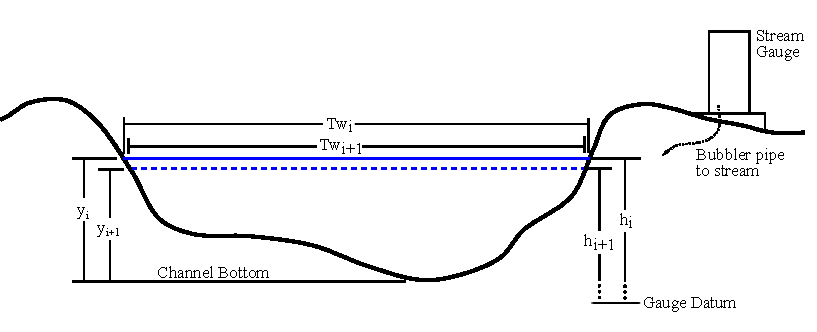
\includegraphics[width=6in]{Figures/LineDiagram/XSection}
	\caption[Average river segment cross-section area change.]{Average river segment cross-section area change.}
	\label{fig:XSArea}
\end{figure}
\begin{figure}
	\centering
		\includegraphics[width=6.5in]{"Figures/LineDiagram/Trapezoid"}
		\caption[River cross-section area change diagram.]{River cross-section area change diagram.}
		\label{fig:XSTrapezoid}
\end{figure}

\begin{align}
	\frac{\Delta A_i}{\Delta t}= & \overline{Tw}\cdot \Delta y \nonumber \\
	\frac{\Delta A_i}{\Delta t} = & \frac{Tw_t + Tw_{t-1}}{2} \cdot \left( y_{t-1} - y_t \right) \label{eq:XSArea}
\end{align}
\begin{tabular}{r p{5.5in}}
	Where: & \\
	$_t$ = & Current time step. \\
	$_{t-1}$ = & Previous time step. \\
	$\displaystyle \frac{\Delta A_i}{\Delta t}$ = & Cross-section area change at river section $ i $ between time steps.\\
	$\overline{Tw}$ = & Average river top width.\\
	$\Delta y$ = & Change in flow depth from the previous time step. \\
	$Tw$ = & River top width. \\
	$y$ = & River flow depth. \\
\end{tabular}\\

Figure \ref{fig:XSArea} shows a simplified river cross section at a stream gauge location.  As previously discussed, stream gauges do not hold the channel bottom as their datum.  They have an arbitrarily fixed datum that does not move unless reset by the gauge owner.  The difference between the stream gauge datum and the channel bottom is corrected using a constant correction factor calculated from the river survey.  The gauge datum does not have a known marker where the elevation could be directly measured.  Instead, the surveyed water surface elevation was recorded at the gauge location on both sides of the channel.  The flow depth value was calculated by finding the difference between the surveyed average water surface elevation and the surveyed channel bottom elevation.  The flow depth was then compared to the stream gauge height reported for the same date and time as when the water surface elevation was surveyed.  The difference between the reported value and the average of the surveyed values was taken as the correction factor for the gauge.  This procedure was repeated for each gauge.

Flow depth values as reported by the USGS and CDWR are measured values with an associated probability range as calculated in equation \ref{eq:uncertainty3}.  The uncertainties are applied as shown in equation \ref{eq:herror1}.  A correction factor ($ C_{i} $) is applied to each reported gauge depth to correct for the difference between the gauge datum and the channel bottom as measured during the channel cross-section survey.  Two separate uncertainties are applied.  $ \varepsilon_{h1} $ is the uncertainty distribution as described by the gauge owner.  This uncertainty is reported by both the USGS and CDWR as being normally distributed with extreme values at \SI{0.01}[$\pm$]{\foot} (\SI{0.003}[$ \pm $]{\meter}) \parencite{USGSPL89}.  The second uncertainty term, $ \varepsilon_{h2} $, is the result of personal observation of the river channel along its entire length.  This term describes the variability in flow depth.  It was observed that the channel depth did not vary greatly along most of its length.  There were particular areas where there were deeper pools, but these areas were noted to be more prone to ponding during low flow.  It is assumed that the average effective flow depth only varies within a normal distribution with limits of \SI{0.076}[$ \pm $]{\meter} (\SI{0.25}[$ \pm $]{\foot}).  There is the possibility that $\varepsilon_{h1}$ could cause the storage change between the time steps to change from a storage gain to a storage loss, or vise versa.  This is acceptable as it is within the measurement limits of the instruments.  Once $h+\varepsilon_{h1}$ has been calculated for the two successive time steps, the relationship between the two time steps is fixed.  If the river segment flow depth rises between time steps after this calculation, then that relationship must continue throughout the rest of the volume change calculation.  To facilitate this, it is assumed that $\varepsilon_{h2}$ does not vary significantly within the study time frame and does not vary within a realization.  The Arkansas River channel is sufficiently stable between consecutive days that this assumption is valid.  A new $\varepsilon_{h2}$ is drawn for each realization and remains constant for all time steps within the study time frame.
\begin{equation}
	y_{i,t}=h_{i,t}+C_{i}+\varepsilon_{h1}+\varepsilon_{h2}
	\label{eq:herror1}
\end{equation}
\begin{tabular}{r p{5.5in}}
	Where: & \\
	$y_{i,t}$  & = Section $ i $ modeled average daily flow depth at time $ t $.\\
	$h_{i,t}$  & = Section $ i $ reported average daily river gauge height at time $ t $.\\
	$ C_{i} $ & = Section $ i $ river gauge height to flow depth correction term.\\
	$\varepsilon_{h1}$ & = Reported river gauge height data uncertainty.\\
	$\varepsilon_{h2}$ & = Estimated flow depth uncertainty.\\
\end{tabular}\\

Since the two uncertainty terms are both normal and additive to flow depth, they were added to produce a new normal distribution with mean equal to the sum of the means of the two distributions and standard deviation equal to the sum of the standard deviations of the two distributions.  This additional step was taken to improve model calculation speed and to reduce the possible error of producing a total flow depth error that would cause a flow depth outside of the accepted range of \SIrange{0.153}{1.53}{\meter} (\SIrange{0.5}{5}{\foot}).  The uncertainty distributions $ \varepsilon_{h1} $ and $ \varepsilon_{h2} $ are not dependent on location, therefore all flow depth calculations draw from the same distribution.  The normal distribution resulting from the addition of the $ \varepsilon_{h1} $ and $ \varepsilon_{h2} $ has a mean of zero and standard deviation of \SI{0.00707}{\meter} (\SI{0.02032}{\foot}) (Equation \ref{eq:herror2}).  
\begin{equation}
	y_{i,t}=h_{i,t}+C_{i}+\mathcal{N} \left( \mu=0m, \sigma=0.00707m \right)
	\label{eq:herror2}
\end{equation}

River top width $ \left( Tw \right)  $ is calculated using equation \ref{eq:Tw1}  \parencite{Buhman2002,Gates1996}. The river channel does not have a fixed cross-section along it's length, therefore, the fitting parameters, $ \beta_1 $ and $ \beta_2 $ are not constant, but are from distributions of  $ \beta_1 $ and $ \beta_2 $.  Equation \ref{eq:Tw1} and the data from each survey cross-section was used to calculate a best fit equation using non-linear least squares regression.  Regression results for each cross-section are presented in Table \ref{tab:alphabetavals}.  There are an insufficient number of cross sections within each river segment to provide a statistically significant sample.  This means that there is insufficient data available to generate independent fitting equations for each river segment.  Therefore, the $ \beta_1 $ and $ \beta_2 $ values from each cross-section were combined to determine the distribution of $ \beta_1 $ and $ \beta_2 $ for the entire river reach.  The combined distributions were tested to determine the best fit parametric distribution using the previously described method.  The best fit distributions for $ \beta_1 $ and $ \beta_2 $ are presented in table \ref{tab:TwFitting}.  $ \beta_1 $ and $ \beta_2 $ values were analyzed for correlation which was found to be insignificant with a Pearson R value of 0.17.  Visual analysis of the data points showed that there was no distinguishable pattern.  Future cross-section surveys will expand the data set and may show that there is a correlation between $ \beta_1 $ and $ \beta_2 $, but the available data does not support that conclusion.  Also presented in Table \ref{tab:TwFitting} is the best fit distribution for the residuals.  These distributions and the distributions for $ \beta_1 $ and $ \beta_2 $ were analyzed to determine the best fit distribution using the methodology described in Section \ref{sec:ErrorAndUncertainty}.

\begin{equation}
	\label{eq:Tw1}
	Tw_{i,t} = \beta_1 y_{i,t} ^{\beta_2} + \varepsilon_{Tw}
\end{equation}
\begin{tabular}{r p{5in}}
	Where: & \\
	$ Tw_{i,t} $ =& River segment $ i $ average daily top width at time step $ t $.\\
	$ y_{i,t} $ =& Calculated segment $ i $ average daily flow depth at time step $ t $ calculated using equation \ref{eq:herror1}.\\
	$ \beta_1 $ and $ \beta_2 $ =& fitting parameter distributions.\\
	$ \varepsilon_{Tw} $=& Calculated average daily flow depth uncertainty.\\
\end{tabular}\\

\begin{table}[htbp]
	\centering
	\caption[Arkansas River segment top width estimating coefficients.]{Arkansas River segment top width estimating coefficients.}
	\label{tab:alphabetavals}
	\begin{tabular}{cccccc}
		\toprule
		Study & River & Cross- & \multicolumn{2}{c}{Fitting Parameter} & Root Mean\\ \cmidrule(l{0.5em}r){4-5}
		Region & Segment & Section & $\beta_1$ & $\beta_2$ & Squared Error\\
		\toprule
		\multirow{21}{*}{USR}& \multirow{4}{*}{A} 		& 1 & 219.1	& 0.5098	& 21.57	\\
		& 						& 2 & 197.5 & 0.01573 &	0.07938 \\
		&						& 3 & 205.2 & 0.7734 & 32.05 \\
		&  						& 4 & 211.5 & 0.008948 & 0.2069 \\ \cmidrule(l{0.5em}r){2-6}
		&  \multirow{3}{*}{B} & 5 & 59.4 & 0.9835 & 0.5002 \\ 
		&						& 6 & 202 & 0.1382 & 12.48 \\ 
		&  						& 7 & 53.99 & 1.197 & 2.412 \\ \cmidrule(l{0.5em}r){2-6}
		& \multirow{5}{*}{C} & 10 & 141 & 0.5465 & 10.92 \\
		&						& 11 & 187.2 & 0.5697 & 7.784 \\
		&						& 12 & 277.9 & 0.01398 & 0.2358	\\ 
		& 						& 13 & 116.5 & 1.536 & 27.5 \\
		&						& 14 & 110 & 0.917 & 1.986 \\ \cmidrule(l{0.5em}r){2-6}
		&\multirow{7}{*}{D}	& 16 & 49.37 & 1.115 & 1.5171 \\ 
		&						& 17 & 57.68 & 1.288 & 1.469 \\
		&						& 18 &116.4 & 0.5197 & 17.42 \\
		&						& 19 & 58.35 & 0.3868 & 6.382 \\ 
		&						& 21 & 141 & 0.07095 & 0.7172 \\
		&						& 22 & 63.82 & 0.6103 & 1.132	\\
		&						& 23 & 109.3 & 0.07456 & 0.4762 \\ \cmidrule(l{0.5em}r){2-6}
		&	E				& 26 & 47.62 & 0.1682 & 0.5901 \\
		\midrule
		\multirow{13}{*}{DSR}& \multirow{7}{*}{F} & 1 & 22.48 & 0.4006 & 0.8139\\
		&						& 2 & 41.61 & 1.390 & 3.953\\
		&						& 3 & 29.82 & 0.2265 & 1.821\\
		& 						& 4 & 21.46 & 0.3801 & 2.541\\
		&						& 5 & 22.78 & 0.8004 & 5.715\\
		&						& 6 & 26.21 & 0.4153 & 1.681\\
		&						& 7 & 41.92 & 1.487 & 3.299\\ \cmidrule(l{0.5em}r){2-6}
		& \multirow{7}[2]{*}{G} & 8 & 23.49 & 1.504 & 2.344\\
		&						& 9 & 33.54 & 1.106 & 3.676\\
		&						& 10& 28.03 & 0.5790 & 2.003\\
		&						& 11& 24.16 & 0.2103 & 1.693\\
		&						& 12& 24.74 & 0.8992 & 2.617\\
		&						& 13& 52.68 & 1.1850 & 5.757\\
		&						& 14& 24.18 & 0.4764 & 0.9259\\
		\bottomrule
	\end{tabular}\\
\end{table}

Non-linear regression models were used only when the specific model form, determined from known physical or geometrical relationships, was non-linear.  R-squared values were not used to determine goodness-of-fit for non-linear regression models since they can have valid R-squared values that are negative or greater than one \parencite{spiess2010} and as such are outside of the boundary for comparing linear models.  Pseudo or modified r-squared calculations are available, yet these computations result in values that are comparable to the r-squared value for linear models, but have slightly different interpretations.  Since non-linear regression models were used only when specific model forms could be predetermined, there was no need to compare different model forms estimating the same result.

Goodness-of-fit for non-linear regressions used in this thesis are purely for informational purposes.  Since all non-linear models were based on known relationships, goodness-of-fit values only serve to show how well the data fits the model.  In order to define non-linear regression model goodness-of-fit, the root mean squared error (RMSE) value was calculated.  The RMSE represents the standard deviation of the differences between the predicted and observed values.  The RMSE is scale dependent as the units are the same as the observed value.  The RMSE is also known as the standard deviation.  This would cause an issue if models for different observed value units and scales were compared against each other.  In this study, non-linear regression models are only used to estimate the cross-sectional width of a river segment and to estimate the selenium concentration at one location.  Since all cross-section analyses use the same measurement units, this allows us to compare the residual errors associated with the various cross sections without needing to consider scale or units.

The results of the top width equation for each cross-section, generated through non-linear regression, was compared to the observed results to visually compare the goodness-of-fit for each cross-section.  Figure \ref{fig:exampleTwVsH} is an example
\begin{figure}[htbp]
	\centering
	\includegraphics[width=6in]{"Figures/Results_USR/Stochastic/Survey Tw vs H-Section 1"}
	\caption[Example Flow Depth vs. River Top Width Relationship.]{Example Flow Depth vs. River Top Width Relationship.  The non-linear best fit line of the form in Equation \ref{eq:Tw1} is red.  The values are the two non-linear regression fitting parameters ($\beta_1$ and $\beta_2$) and the residual standard error for the fitting equation ($\sigma$).  Similar figures for all cross-sections are found in the appendix.}
	\label{fig:exampleTwVsH}
\end{figure}

\begin{table}[htbp]
	\centering
	\caption[River top width fitting parameter distributions.]{River top width fitting parameter distributions.}
	\label{tab:TwFitting}
	\begin{tabular}{ccccc}
		\toprule
		Study                & Fitting   & \multicolumn{3}{c}{Best Fit Distribution} \\ \cmidrule(r{.5em}l){3-5}
		Reach                & Parameter & Dist. Shape      & p1*        & p2*       \\
		\toprule
		\multirow{3}{*}{USR} & $\beta_1$ & logistic         & 16.8       & 7.53      \\
		& $\beta_2$ & log-normal       & -1.27      & 1.57      \\
		& Residual  & logistic         & 1.99       & 0.99      \\
		\midrule
		\multirow{3}{*}{DSR} & $\beta_1$ & logistic         & 28.2       & 4.84      \\
		& $\beta_2$ & log-normal       & -0.43      & 0.65      \\
		& Residual  & log-normal       & 0.87       & 0.57      \\
		\bottomrule
		\multicolumn{5}{l}{{\footnotesize * Distribution fitting parameters.  For logistic, p1=location }}\\
		\multicolumn{5}{l}{\footnotesize{and p2=scale.  For log-normal, p1=mean of the log scale }}\\
		\multicolumn{5}{l}{\footnotesize{and p2=standard dev. of the log scale}}\\
	\end{tabular}\\
\end{table}

Values $\beta_1$ and $\beta_2$ are drawn from probability distributions.  Calculated flow depth and river top width data pairs were used to determine the distributions from which $\beta_1$ and $\beta_2$ in equation \ref{eq:Tw1} were drawn.  These distributions were developed using non-linear, least-squares regression.  Values below \SI{0.15}{\meter} (\SI{0.5}{\foot}) were removed from the regression analysis.  Flow values below this depth are not common and it was determined that these points would not allow for an accurate representation of the flow depth to river top width relationship for the range of known flow depths.  Values above \SI{1.52}{\meter} (\SI{5.0}{\foot}) were also removed from the regression analysis.  Flow depths above this depth are above the banks of the primary river channel and are within the inner flood plain.  Table \ref{tab:alphabetavals} gives the resulting $\beta_1$ and $\beta_2$ values for each surveyed cross-section.  Figure \ref{fig:exampleTwVsH} is an example of the surveyed flow depth and river top width relationships and the derived non-linear relationship for cross-section 1 in river segment A of the USR.  Similar relationship plots for the other surveyed cross-sections are found in the appendix. 

Figure \ref{fig:B1B2} shows the distributions of $\beta_1$ and $\beta_2$ values and the various best-fit distributions in both the USR and DSR.  Logistic, normal, exponential, Weibull, and log-normal distributions were fitted to the data.  Vertical tick marks in the x-axis margin are at the data values.  Kernel density estimations were used as an alternative means to graphically represent the data density.  

\begin{figure}[htbp]
\centering
\begin{subfigure}{0.5\textwidth}
	\centering
	\includegraphics[width=0.9\linewidth]{"Figures/Results_USR/Stochastic/USR B1 Dist"}
	\caption{USR $\beta_1$}
\end{subfigure}%
\begin{subfigure}{0.5\textwidth}
	\centering
	\includegraphics[width=0.9\linewidth]{"Figures/Results_USR/Stochastic/USR B2 Dist"}
	\caption{USR $\beta_2$}
\end{subfigure}
\begin{subfigure}{0.5\textwidth}
	\centering
	\includegraphics[width=0.9\linewidth]{"Figures/Results_DSR/Stochastic/DSR B1 Dist"}
	\caption{DSR $\beta_1$}
\end{subfigure}%
\begin{subfigure}{0.5\textwidth}
	\centering
	\includegraphics[width=0.9\linewidth]{"Figures/Results_DSR/Stochastic/DSR B2 Dist"}
	\caption{DSR $\beta_2$}
\end{subfigure}\\
\caption[$Tw$ Versus $h$ Fitting Parameter $\beta_1$ and $\beta_2$ Distributions.]{$Tw$ Versus $h$ Fitting Parameter $\beta_1$ and $\beta_2$ Distributions.  The black dashed line is a kernel density plot representing a histogram where the bin size approaches zero.  The colored curves are the best fit for the particular distribution type.  Vertical tick marks in the x-axis are at the data values.}
\label{fig:B1B2}
\end{figure}

The resulting river shape parameter distributions are valid for the river reach for which they were calculated.  Each river segment draws values from the shape parameter distributions independently.  Only one pair of shape parameters is drawn for each realization.  It is assumed that the river geometry does not significantly change within the study time frame.  Channel variability is modeled between the realizations.

Residuals from the non-linear regression analyses were combined into a single data set for uncertainty analysis.  Combining this data set was a logical step following the combination of the data that generated the residuals.  Residuals were tested using the same tools and techniques used to test the river shape parameter distributions.  USR and DSR channel shape residuals were found to have a log-normal distribution.  Figure \ref{fig:B1B2 Error} presents the residuals distribution analyses for the USR and DSR.  These figures are of the same type as those used to analyze the river shape parameter distributions, figure \ref{fig:B1B2}.

\begin{figure}[htbp]
\centering
\begin{subfigure}{0.5\textwidth}
	\centering
	\includegraphics[width=0.9\linewidth]{"Figures/Results_USR/Stochastic/USR AB Error Dist"}
	\caption{USR Residuals}
\end{subfigure}%
\begin{subfigure}{0.5\textwidth}
	\centering
	\includegraphics[width=0.9\linewidth]{"Figures/Results_DSR/Stochastic/DSR AB Error Dist"}
	\caption{DSR Residuals}
\end{subfigure}\\
\caption[$Tw$ Versus $H$ Residuals Distribution.]{$Tw$ versus $H$ Residuals Distribution.  The black dashed line is a kernel density plot representing a histogram where the bin size approaches zero.  The colored curves are the best fit for the particular distribution type.  Vertical tick marks in the x-axis are at the data values.}
\label{fig:B1B2 Error}
\end{figure}

Residuals are the collection of the difference between the calculated regression model values and the measured values.  Collectively, the distribution of the residuals describe the uncertainty of the regression model.  In this case, the distribution of residuals describe the top width estimating uncertainty $ \varepsilon_{Tw} $.  Residuals should be tested for heteroskedasticity to determine if the model does not adequately predict the data.  Heteroskedasticity is the condition where the variability of a variable, in this case the residuals, is unequal across the range of the values and is usually indicative of under specification of the model.  There are many tests for heteroskedasticity, but the most powerful is visual analysis of the plot of the residuals against the fitted, or calculated, values.  When a small number of values is used to perform the regression, visual and computational analysis becomes difficult since patterns may appear that don't truly exist or patterns may not appear where they do exist.  When heteroskedasticity was evident during model creation, the model was modified to remove the heteroskedasticity.  Other methods are available to account for heteroskedasticity, but the most strongly recommended is model modification.  Determining the parametric distribution that best fits the regressions is performed using the method described in section \ref{sec:ErrorAndUncertainty}.  Both visual and goodness-of-fit tests were applied to all residual regression analyses.

Results from the individual regression and residuals analyses are plotted with the source data to visually determine if the resulting best fit estimating equation or residuals distribution suitably fit the source data.  An example of one of these figures is Figure \ref{fig:exampleTwVsH} which plots a best fit regression equation alongside the source data.  Figure \ref{fig:B1B2 Error} is representative of how the residual analysis results are visually analyzed.  The best fit of several different distribution shapes are plotted over the histogram and KDE of the residuals or source data.  These types of figures are used throughout the analysis to visually verify that the calculated regression models and best-fit distributions actually fit the data.

Results from deterministic and stochastic models are presented throughout this thesis.  While both model types present results from the same source data, stochastic models, as previously discussed, also include uncertainty in many forms.  Stochastic model results are complex.  They are time-series models where each time step is an independent distribution of the results.  Figure is a very simple representation of a time-series.  The top sub-figure shows a sine curve which represents the deterministic model.  The second sub-figure shows one realization of the stochastic model which is the deterministic model with uncertainty added at each time step.  For this example, the uncertainty is normally distributed within the time step.  The third sub-figure is 500 independent realizations shown on top of each other.  The fourth sub-figure shows the 500 realizations with three calculated lines representing stochastic model summary statistics time-series.

\begin{figure}[htbp]
	\centering
	\includegraphics[width=0.9\linewidth]{"Figures/LineDiagram/TSDescription"}
	\caption[Stochastic model graphical results presentation description.]{Stochastic model graphical results presentation description.  The top sub-figure represents a simple deterministic time-series model.  The second sub-figure represents a single stochastic time-series model.  The third sub-figure represents 500 stochastic time-series.  The fourth sub-figure shows the 500 stochastic time-series with the three stochastic model summary statistics time-series.  The top line is the 97.5th percentile time-series, the middle line is the mean time-series, and the bottom line is the 2.5th percentile time-series.}
	\label{fig:StochExample}
\end{figure}

The middle line is the time-series that represents the mean value calculated for each time-step.  This is the stochastic model mean time-series.  The top and bottom lines are the 97.5th and 2.5th percentile calculated for each time step.  These are the stochastic model 97.5th percentile time-series and stochastic model 2.5th percentile time-series, respectively.  Collectively, these three time-series are called stochastic model summary statistics time-series.  These three time-series show how the results and range of possible results vary with time.  All stochastic time-series graphs present only the three stochastic model summary statistics time-series.  Values outside of these are not plotted so as to improve understanding and readability of the graphical results

Presenting individual values for stochastic model results requires further summary statistics of the calculated stochastic model summary statistics time-series.  Without this further reduction, results would contain large quantities of values which are very difficult to present.  The mean, 97.5th percentile, and 2.5th percentile are calculated for each of the summary statistics time-series to provide more readable results.  The summary statistics for each of the stochastic model summary statistics time-series indicate the most likely value and the range of possible values as presented in the example in Table \ref{tab:ExStochResultsTable}.  In this table, each row of the bottom portion of the table presents one of the stochastic model summary statistic time-series results.  In this example, values '$ g $', '$ h $', and '$ i $' are the summary statistics for the stochastic model mean time-series.

Table \ref{tab:ExStochResultsTable} also includes the deterministic time-series summary statistics values.  These values are the 2.5th percentile, mean, and 97.5th percentile calculated from the deterministic model results and are presented in the upper half of the table.  The deterministic model time-series summary statistics should be approximately the same as the stochastic model mean time-series summary statistics, which are values $ g $,  $ h $, and $ i $ in the lower half of the table.  This statement should be true if the deterministic model is a possible realization of the stochastic model and if the distribution of the combined uncertainties in the stochastic model are approximately normally distributed.

\begin{table}[htbp]
	\centering
	\caption[Example deterministic and stochastic model numerical results.]{Example deterministic and stochastic model numerical results.  The single row on on the deterministic model side presents the summary statistics for the deterministic model (values $ a $, $ b $, and $ c $).  Each row on the stochastic model side presents the results for a specific stochastic model summary time-series.  All values are presented in common units.  The Pearson Correlation value ($ m $) is calculated between the deterministic model time-series and the stochastic model mean time-series values at each time-step in the models.}
	\label{tab:ExStochResultsTable}
	\begin{tabular}{C{1.25in} C{1.4in} C{1.4in} C{1.4in}}
		\toprule
		\multicolumn{4}{l}{\textbf{Deterministic Model Time Series}} \\
		& 2.5th      & \multirow{2}{*}{Mean} & 97.5th   \\
		& Percentile &                       &            Percentile \\ \cmidrule(r{.5em}l){2-4}
		& a			& b			&  c         \\
		\toprule
		\multicolumn{4}{l}{\textbf{Stochastic Model Summary Statistics Time Series}} \\ 
		& 2.5th      & \multirow{2}{*}{Mean} & 97.5th\\
		& Percentile &                       & Percentile \\ \cmidrule(r{.5em}l){2-4}
		97.5th Percentile	& d			& e			& f \\
		Mean						& g			& h			& i \\
		2.5th Percentile	& j			& k			& l \\
		\bottomrule
		\multicolumn{4}{l}{Pearson Correlation = m}
	\end{tabular}\\
\end{table}

One goal of stochastic modeling is to have a deterministic model that resides within the stochastic.  If the deterministic model isn’t a possible realization of the stochastic model, then there are significant stochastic model issues that need to be addressed.  Ideally, the stochastic model mean time-series at each time step should be close to the deterministic model at that same time step.  To determine if this relationship is true, the Pearson correlation between the stochastic model mean time-series and the deterministic model was calculated and is included at the bottom of Table \ref{tab:ExStochResultsTable}.  Calculating the Pearson correlation requires assuming the two compared data sets are continuous and are linearly related.  All input values and results in this thesis are continuous, either from zero to $ +\inf $ or between $ \pm \inf $.

Correlation values only provides a numerical value to describe the relationship between two values or data sets.  It does not imply causality or linearity.  We can infer causality because the deterministic model is a subset of the stochastic model.  In fact, the deterministic model was used to create the stochastic model.  We cannot infer linearity.  Figure \ attempts to answer the linearity issue through visual analysis.  The black dots are the comparison of the stochastic mean time-series and the deterministic model.  The red and blue does are the comparison of the stochastic 97.5th and 2.5th percentile time-series as compared to the deterministic model, respectively.  The solid black line follows the equation y=x.  This is where all of the black dots should lie if the stochastic mean time-series and deterministic models were in perfect agreement.  The dashed line is the quadratic best fit line through the stochastic mean time-series.

\begin{figure}[htbp]
	\centering
	\includegraphics[width=0.9\linewidth]{"Figures/Results_USR/Stochastic/S-D Comparison-M Mass Flow"}
	\caption[Example scatterplot comparing the deterministic model time-series and stochastic model mean time-series results.]{Example scatterplot comparing deterministic model time-series and stochastic model mean time-series results.  The solid line is drawn such that $ y=x $.  The dashed line is the best-fit quadratic equation between the deterministic model time-series and the stochastic model mean time-series and the equation is in the top right. The Pearson Correlation is the top left number.}
	\label{fig:CorrelationExample}
\end{figure}

River segment B in the USR does not have a flow gauge within its boundaries and therefore has no reported flow depths. This segment has an additional irrigation diversion check structure within its boundaries, thereby sub-dividing segment B into two sub-segments, each with its own ungauged flow depth.  Due to segment B being the shortest, composing only 3.9\% of the USR's total length, and the additional variability of the possible flow depth, the average daily flow depth within segment B is taken as the mean of the reported flow depths in segment A and C.  Top width and volume change calculation follows the previously described methodology.

\clearpage
The time-series plots of all four stochastic geometric parameters for each study region river section segment is presented in Figures \ref{fig:GeoTS_US} and \ref{fig:GeoTS_DS} for the USR and DSR, respectively.  The black lines indicate the stochastic model mean time-series.  The blue band indicates the 95\% central inter-percentile range (CIR) of the stochastic values as defined by the stochastic model 2.5th percentile time-series and the stochastic model 97.5th percentile time-series.  The red dashed line in the flow depth portion of the figure indicates the reported flow depth values.  It is plotted under the stochastic model mean time-series line and as such is only visible when either the stochastic model mean time-series value was not calculated due to missing data or when the two values deviate.

\subfiguretop
\begin{landscape}
	\begin{figure}
		\begin{subfigure}{0.7\textwidth}
			\centering
			\includegraphics[width=\tableCustomSize]{"Figures/Results_USR/Stochastic/G TS A"}
			\subcaption*{Segment A}		
			\label{sub:GeoTS_A}
		\end{subfigure}%
		\begin{subfigure}{0.7\textwidth}
			\centering
			\includegraphics[width=\tableCustomSize]{"Figures/Results_USR/Stochastic/G TS B"}
			\subcaption*{Segment B}
			\label{sub:GeoTS_B}
		\end{subfigure}\\
	\caption[USR and DSR stochastic geometric parameter time-series.]{USR and DSR stochastic geometric parameter time-series. The black lines indicate the stochastic model mean time-series.  The blue band indicates the 95\% central inter-percentile range (CIR) of the stochastic values.  The red dashed line in the flow depth portion of the figure indicates the reported flow depth values.}
	\label{fig:GeoTS_US}
	\end{figure}
\end{landscape}

\subfiguremid
\begin{landscape}
	\begin{figure}
		\begin{subfigure}{0.7\textwidth}
			\centering
			\includegraphics[width=\tableCustomSize]{"Figures/Results_USR/Stochastic/G TS C"}
			\subcaption*{Segment C}
			\label{sub:GeoTS_C}	
		\end{subfigure}%
		\begin{subfigure}{0.7\textwidth}
			\centering			
			\includegraphics[width=\tableCustomSize]{"Figures/Results_USR/Stochastic/G TS D"}
			\subcaption*{Segment D}
			\label{sub:GeoTS_D}
		\end{subfigure}\\
		\caption{USR and DSR stochastic geometric parameter time-series.}
	\end{figure}
\end{landscape}

\subfiguremid
\begin{landscape}
	\begin{figure}
		\begin{subfigure}{0.7\textwidth}
			\centering
			\includegraphics[width=\tableCustomSize]{"Figures/Results_USR/Stochastic/G TS E"}
			\subcaption*{Segment E}
			\label{sub:GeoTS_E}	
		\end{subfigure}\\
		\caption{USR and DSR stochastic geometric parameter time-series.}
	\end{figure}
\end{landscape}

\subfiguretop
\begin{landscape}
	\begin{figure}
		\begin{subfigure}{0.7\textwidth}
			\centering
			\includegraphics[width=0.9\textwidth]{"Figures/Results_DSR/Stochastic/G TS F"}
			\subcaption*{Segment F}		
			\label{sub:GeoTS_F}
		\end{subfigure}%
		\begin{subfigure}{0.7\textwidth}
			\centering
			\includegraphics[width=0.9\textwidth]{"Figures/Results_DSR/Stochastic/G TS G"}
			\subcaption*{Segment G}
			\label{sub:GeoTS_G}
		\end{subfigure}
		\caption[DSR stochastic geometric parameter time-series.]{DSR stochastic geometric parameter time-series. The black lines indicate the stochastic model mean time-series.  The blue band indicates the 95\% central inter-percentile range (CIR) of the stochastic values.  The red dashed line in the flow depth portion of the figure indicates the reported flow depth values.}
		\label{fig:GeoTS_DS}
	\end{figure}
\end{landscape}

Figures \ref{fig:GeoTS_US} and \ref{fig:GeoTS_DS} were analyzed to verify that direct correlations existed between the flow depth and the calculated geometric parameters.  Top width and surface area should increase and decrease in proportion with the increase and decrease in flow depth.  Volume changes are based on two flow depth values and do not have a direct correlation to the flow depth displayed in the figure.  All of the river sections show the correct correlations between flow depth and the calculated river geometric parameters.

Tables \ref{tab:SegmentSurfaceArea_USR} and \ref{tab:SegmentSurfaceArea_DSR} present the river segment average daily surface area deterministic model time-series and stochastic model summary statistic time-series results for the USR and DSR, respectively.  Summary results for river segment average daily flow depth and river segment average daily top width are not included as they are not direct precursors to the final model results.  The surface area is directly used for precipitation and evaporation calculations.

\subtabletop
\begin{table}[htbp]
	\centering
	\caption[USR river segment surface area deterministic and stochastic model numerical results.]{USR river segment surface area deterministic and stochastic model numerical results.  Values are in hectares (\si{\hectare}) with values in parentheses in acres (\si{\acre}).}
	\label{tab:SegmentSurfaceArea_USR}
	\begin{subtable}{\textwidth}
		\centering
		\subcaption*{USR river segment A}
		\input{"Tables/tableAreaA.txt"}
	\end{subtable}\\
	\tablevspace
	\begin{subtable}{\textwidth}
		\centering
		\subcaption*{USR river segment B}
		\input{"Tables/tableAreaB.txt"}
	\end{subtable}\\
\end{table}

\subtablemid
\begin{table}[htbp]
	\centering
	\caption{USR river segment surface area deterministic and stochastic model numerical results.}
	\begin{subtable}{\textwidth}
		\centering
		\subcaption*{USR river segment C}
		\input{"Tables/tableAreaC.txt"}
	\end{subtable}\\
	\tablevspace
	\begin{subtable}{\textwidth}
		\centering
		\subcaption*{USR river segment D}
		\input{"Tables/tableAreaD.txt"}
	\end{subtable}\\
\end{table}

\subtablemid
\begin{table}[htbp]
	\centering
	\caption{USR river segment surface area deterministic and stochastic model numerical results.}
	\begin{subtable}{\textwidth}
		\centering
		\subcaption*{USR river segment E}
		\input{"Tables/tableAreaE.txt"}
	\end{subtable}\\
\end{table}

\subtabletop
\begin{table}[htbp]
	\centering
	\caption[DSR river segment surface area deterministic and stochastic model numerical results.]{DSR river segment surface area deterministic and stochastic model numerical results.  Values are in hectares (\si{\hectare}) with values in parentheses in acres (\si{\acre}).}
	\label{tab:SegmentSurfaceArea_DSR}
	\begin{subtable}{\textwidth}
		\centering
		\subcaption*{DSR river segment F}
%		\input{"Tables/tableAreaF.txt"}
	\end{subtable}\\
	\tablevspace
	\begin{subtable}{\textwidth}
		\centering
		\subcaption*{DSR river segment G}
%		\input{"Tables/tableAreaG.txt"}
	\end{subtable}\\
\end{table}

Every one of these tables shows that the stochastic model tends to underestimate the river segment water surface area by approximately 38\% in the USR and XX\% in the DSR.  The correlation values indicate that the deterministic model time-series and stochastic model mean time-series are highly correlated.  The corresponding correlation scatter-plots show that the relationships are linear.  This is due to the way the river section average daily top width was estimated for the deterministic models.  Since $ \beta_1 $ and $ \beta_2 $ are drawn from distributions and the deterministic model requires that none of the input values are variable, the most likely values from the respective distributions were chosen as the fixed values.  The $ \beta $ values from both study reaches are not normal, therefore the most likely value is not the mean and the values are not evenly distributed on either side of the likely value.  The skewness of the $ \beta $ values is represented in the stochastic model.  Calibrating the deterministic models to find the $ \beta $ values that approximate the stochastic model defeats the purpose of the deterministic model, which is to estimate the most likely values.  Sensitivity analysis which is discussed later, will show whether or not the river section average daily surface area values are significant enough to warrant the effort required to calibrate them to the stochastic model.

Tables \ref{tab:SegmentVolumeChange_USR} and \ref{tab:SegmentVolumeChange_DSR} present the river segment average daily surface area deterministic model time-series and stochastic model summary statistic time-series results for the USR and DSR, respectively.  Summary results for river segment average daily flow depth and river segment average daily top width are not included as they are not direct precursors to the final model results.  The surface area is directly used for precipitation and evaporation calculations.
\\
\subtabletop
\begin{table}[htbp]
	\centering
	\caption[USR river segment volume change deterministic and stochastic model numerical results.]{USR river segment volume change deterministic and stochastic model numerical results.  Values are in hectare-meters (\si{\hectare\meter}) and the values in parentheses are in acres (\si{\acre}).}
	\label{tab:SegmentVolumeChange_USR}
	\begin{subtable}{\textwidth}
		\centering
		\subcaption*{ $\displaystyle\frac{\Delta S_{A}}{\Delta t} $ }
		\input{"Tables/tableVolumeA.txt"}
	\end{subtable}\\
	\tablevspace
	\begin{subtable}{\textwidth}
		\centering
		\subcaption*{ $\displaystyle\frac{\Delta S_{B}}{\Delta t} $ }
		\input{"Tables/tableVolumeB.txt"}
	\end{subtable}\\
\end{table}	
\subtablemid
\begin{table}[htbp]
	\centering
	\caption{USR river segment volume change deterministic and stochastic model numerical results.}
	\begin{subtable}{\textwidth}
		\centering
		\subcaption*{ $\displaystyle\frac{\Delta S_{C}}{\Delta t} $ }
		\input{"Tables/tableVolumeC.txt"}
	\end{subtable}\\
	\tablevspace
	\begin{subtable}{\textwidth}
		\centering
		\subcaption*{ $\displaystyle\frac{\Delta S_{D}}{\Delta t} $ }
		\input{"Tables/tableVolumeD.txt"}
	\end{subtable}\\
\end{table}
\subtablemid
\begin{table}[htbp]
	\centering
	\caption{USR river segment volume change deterministic and stochastic model numerical results.}
	\begin{subtable}{\textwidth}
		\centering
		\subcaption*{ $\displaystyle\frac{\Delta S_{E}}{\Delta t} $ }
		\input{"Tables/tableVolumeE.txt"}
	\end{subtable}\\
	\tablevspace
\end{table}

\subtabletop
\begin{table}[htbp]
	\centering
	\caption[DSR river segment volume change deterministic and stochastic model numerical results.]{DSR river segment volume change deterministic and stochastic model numerical results.  Values are in hectare-meters (\si{\hectare\meter}) and the values in parentheses are in acres (\si{\acre}).}
	\label{tab:SegmentVolumeChange_DSR}
	\begin{subtable}{\textwidth}
		\centering
		\subcaption*{ $\displaystyle\frac{\Delta S_{F}}{\Delta t} $ }
		\input{"Tables/G volF.txt"}
	\end{subtable}\\
	\tablevspace	
	\begin{subtable}{\textwidth}
		\centering
		\subcaption*{ $\displaystyle\frac{\Delta S_{G}}{\Delta t} $ }
		\input{"Tables/G volG.txt"}
	\end{subtable}\\
\end{table}	

The mean of the deterministic model time-series and the mean of the stochastic model mean time-series calculated average daily river segment water volume change are much closer to each other as reported in Tables \ref{tab:SegmentVolumeChange_USR} and \ref{tab:SegmentVolumeChange_DSR}.  The stochastic model mean time-series underestimates the deterministic model time-series values by approximately 47\%.  The difference between the two models in terms of water volume is quite small, less than \SI{1}{\hectare\meter}.  The Pearson correlation values and their associated scatter-plots indicate that the results are strongly linearly related.  The effects of uncertainty on river segment average river daily water volume change is much smaller than the effect on surface area.  As with the surface area results, the significant portion of the difference between the deterministic model time-series and the stochastic model mean time-series is due to the estimation of the most likely values of $ \beta_1 $ and $ \beta_2 $ used in the deterministic models.  At this point, adjusting or calibrating these values such that the results of the deterministic and stochastic models are more closely aligned seems unnecessary.

Figure \ref{fig:USRWaterStore} and \ref{fig:DSRWaterStore} presents the river reach average daily river water storage change deterministic model time-series for the USR and DSR, respectively, as calculated using Equation \ref{eq:storage1}.  The left-hand figure is the deterministic model time-series.  The right-hand figure is the stochastic model results with the black line representing the calculated stochastic model mean time-series and the blue band representing the space between the stochastic model 97.5th percentile time-series and the stochastic model 2.5th percentile time-series.  The minimum and maximum range of values is not presented in this figure.

\begin{figure}[htbp]
\centering
	\begin{subfigure}{0.5\textwidth}
		\centering
		\includegraphics[width=0.9\linewidth]{"Figures/Results_USR/Deterministic/Balance Water - storage"}
		\subcaption*{Deterministic Model.}
		\label{sub:USRWaterStoreD}
	\end{subfigure}%
	\begin{subfigure}{0.5\textwidth}
		\centering
		\includegraphics[width=0.9\linewidth]{"Figures/Results_USR/Stochastic/Balance Water - storage"}
		\subcaption*{Stochastic Model.}
		\label{sub:USRWaterStoreS}
	\end{subfigure}\\
	\caption[USR Arkansas River water storage change contribution to the water model.]{USR Arkansas River water storage change contribution to the water model.}
	\label{fig:USRWaterStore}
\end{figure}

\begin{figure}[htbp]
	\centering
	\begin{subfigure}{0.5\textwidth}
		\centering
		\includegraphics[width=0.9\linewidth]{"Figures/Results_DSR/Deterministic/Balance Water - storage"}
		\subcaption*{Deterministic Model.}
	\end{subfigure}%
	\begin{subfigure}{0.5\textwidth}
		\centering
		\includegraphics[width=0.9\linewidth]{"Figures/Results_DSR/Stochastic/Balance Water - storage"}
		\subcaption*{Stochastic Model.}
	\end{subfigure}\\
	\caption[DSR Arkansas River water storage change contribution to the water model.]{DSR Arkansas River water storage change contribution to the water model.}
	\label{fig:DSRWaterStore}
\end{figure}

Tables xx presents the deterministic model time-series summary statistics and the summary statistics for each of the stochastic model summary statistics time-series for the river reach average daily water storage change in the USR and DSR.

\begin{table}[htbp]
	\centering
	\caption[USR river reach average daily stored water volume change.]{USR river reach average daily stored water volume change.  Values in hectare-meters (\si{\hectare\meter\per\kilo\meter}) and values in parentheses in acre-feet (\si{\acre\foot\per\mile})}
	\label{tab:waterStorage-US}
	\subcaption*{ $\displaystyle\frac{\Delta S_{DSR}}{\Delta t} $ }
	\input{"Tables/USRVolume.txt"}
\end{table}
	\tablevspace
\begin{table}[htbp]
	\centering
	\caption[DSR river reach average daily stored water volume change.]{DSR river reach average daily stored water volume change.  Values in hectare-meters (\si{\hectare\meter\per\kilo\meter}) and values in parentheses in acre-feet (\si{\acre\foot\per\mile})}
	\label{tab:waterStorage-DS}
	\subcaption*{ $\displaystyle\frac{\Delta S_{USR}}{\Delta t} $ }
	\input{"Tables/DSRVolume.txt"}
\end{table}

The figures show that there is a definite seasonal variation in the storage component.  Stored water changes are smallest during the cold months and are increasingly larger during the growing season.  This pattern is caused by irrigation practices in the Lower Arkansas River Basin (LARV).  Stored irrigation water is released from reservoirs upstream of the LARV during the irrigation season as demands require.  During the winter, there is very little to no irrigation occurring.  This, combined with the low precipitation and no additional flow from snow-pack runoff, allow flows in the Arkansas River to reach base flow level when the river is at a natural equilibrium.

This pattern is not as pronounced in the DSR.  This is most likely due to required flow rates being maintained at the Colorado-Kansas border.  With the constant required flow, John Martin Reservoir releases only enough water to meet the required flow rate.  This creates a flow regime that is nearly constant through most of the DSR. 

Deviations are noted during peak irrigation season.  These additional volume changes are most likely due to irrigation flows returning to the Arkansas River from fields irrigated from canal systems that procure and store water upstream of John Martin Reservoir.  The Fort Lyon Storage Canal and Fort Lyon Canal are two examples of canal systems that perform this function.  Water removed from the USR, stored, and added to the DSR is not included in this study.

The distribution of all realizations within each time step was analyzed to determine a distribution type.  This analysis was performed to determine if the assumption that the deterministic model results were representative of the stochastic model.   Testing was performed by comparing K-S statistics for the best fit normal and logistic distributions.  Log-normal, logistic, exponential, gamma, and Weibull distributions were considered, but were not included in this analysis since they do not support the full range of possible values, $ (-\infty, +\infty) $.  The non-included distributions could have been scaled and shifted, but they are still limited in the range of possible values.  In the USR and the DSR, all of the river water volume storage change stochastic model time steps are best fit by a logistic distribution.
  
The mean of the percent difference between the deterministic model time-series and stochastic model mean time-series is very low.  This indicates that the deterministic model is representative of the stochastic model expected value.  The high percent differences at the 2.5th and 97.5th percentile indicate that there is still a large range of uncertainty contained within the stochastic model that the deterministic model cannot replicate.  The deterministic model can be used to determine how changes can affect a reach over a span of time, but using it to estimate values for specific time steps is unwise as the differences noted at individual time steps is too large to account for.
\clearpage{}

\section{Gauged Stream Flows and Diverted Canal Flows}
\label{sec:StreamFlows}

Equation \ref{eq:water1} contains the portion contained in equation \ref{eq:flow1} that describes the sum of all accountable surface water flows entering and leaving a defined reach.  These flows include only the gauged river main stem flows, tributary stream flows, and diverted canal flows.  Most flows are reported as average daily flow rate.  These flow rates, which are measured every 15 minutes, are calculated from the respective gauge's measured instantaneous stage height using stage-discharge tables.  The only exception is with the average daily flow rate reported for the La Junta waste water treatment plant where the average daily flow is converted from the total daily discharge, reported in million gallons per day (mgd).

\begin{equation}
\label{eq:flow1}
\sum Q_{Surface} = \left( Q_{out,DS} + \sum Q_{out} - Q_{in,US} - \sum Q_{in} \right) 
\end{equation}
\begin{tabular}{r p{5.5in}}
	Where: & \\
	$ Q_{Surface} = $ & sum of average daily flow rates in the study region.\\
	$ Q_{in} = $ & flow entering the study reach from a tributary.\\
	$ Q_{out} = $ & flow leaving the study reach to an irrigation canal.\\
	$ Q_{in,US} = $ & flow entering the study reach in the main stem of the river at the upstream end of the reach.\\
	$ Q_{out,DS} = $ & flow leaving the study reach in the main stem of the river at the downstream end of the reach.\\
\end{tabular}\\

Equation \ref{eq:flow1} is expanded as follows to contain all of the measured flows entering or leaving the main stem of the Arkansas River within the USR boundaries.  The subscript for each flow in equation \ref{eq:USRFlow} is the CDWR symbol for a particular gauge site.  See the map in Figure \ref{USRSample} for the gauge locations in the USR.  The flows in this equation are ordered by location along the main stem of the river, from upstream to downstream.
\begin{align}
	\label{eq:USRFlow}
	\sum Q_{Surface,USR} = &~Q_{ARKCATCO} - Q_{HOLCANCO} - Q_{RFDMANCO} - Q_{FLSCANCO} \\
	\nonumber & + Q_{RFDRETCO} + Q_{TIMSWICO} - Q_{FLYCANCO} + Q_{CANSWKCO} \\ 
	\nonumber & + Q_{LAJWWTP} - Q_{CONDITCO} + Q_{HRC194CO} - Q_{ARKLASCO}
\end{align}
Where each subscript is defined as the flow through the gauge described in Table \ref{tab:USRFlow}.  In this table, each of the flow variables in equation \ref{eq:USRFlow}, designated by its CDWR gauge name, is grouped by the type of flow using the variables used in equation \ref{eq:flow1}.

\begin{table}[htbp]
	\centering
	\caption[Description of USR stream flow variables.]{Description of USR stream flow variables.  The CDWR gauge name is the USR model variable sub-script.  The variable group is the category to which the flow belongs.}
	\label{tab:USRFlow}
	\begin{tabular}{c C{1in} p{3.5in}}
		\toprule
		CDWR Gauge & Variable & \multirow{2}{*}{Description}\\
		Name				& Group & \\
		\toprule
		$ ARKCATCO $ & $ Q_{in,US} $ & Arkansas River below the Catlin Canal diversion.\\ 
		$ HOLCANCO $ & $ Q_{out} $ & Holbrook Canal \\
		$ RFDMANCO $ & $ Q_{out} $ & Rocky Ford Canal\\
		$ FLSCANCO $ & $ Q_{out} $ & Fort Lyon Storage Canal\\
		$ RFDRETCO $ & $ Q_{in} $ & Rocky Ford Return Ditch\\
		$ TIMSWICO $ & $ Q_{in} $ & Timpas Creek\\
		$ FLYCANCO $ & $ Q_{out} $ & Fort Lyon Canal\\
		$ CANSWKCO $ & $ Q_{in} $ & Crooked Arroyo\\
		$ LAJWWTP $ & $ Q_{in} $ & Discharge from the La Junta WWTP\\
		$ CONDITCO $ & $ Q_{out} $ & Consolidated Ditch (Jones Ditch)\\
		$ HRC194CO $ & $ Q_{in} $ & Horse Creek at Colorado Highway 194\\
		$ ARKLASCO $ & $ Q_{out,DS} $ & Arkansas River in Las Animas, Colorado\\
		\bottomrule
	\end{tabular}\\
\end{table}

For the DSR, equation \ref{eq:flow1} is expanded as follows to contain all of the measured flows entering or leaving the main stem of the Arkansas River within its boundaries.  The subscript for each flow in equation \ref{eq:DSRFlow} is the CDWR symbol for a particular gauge site.  See the map in Figure \ref{DSRSample} for the gauge locations in the DSR.  The flows in this equation are ordered by location along the main stem of the river, from upstream to downstream.
\begin{align}
	\label{eq:DSRFlow}
	\sum Q_{Surface,DSR} = &~Q_{ARKLAMCO} + Q_{BIGLAMCO} - Q_{BUFDITCO} + Q_{WILDHOCO} \\
	\nonumber & - Q_{FRODITKS} - Q_{ARKCOOKS}
\end{align}
Where each subscript is defined as the flow through the gauge described in Table \ref{tab:DSRFlow}.  In this table, each of the flow variables in equation \ref{eq:DSRFlow}, designated by its CDWR gauge name, is grouped by the type of flow using the variables used in equation \ref{eq:water1}.

\begin{table}[htbp]
	\centering
	\caption[Description of DSR stream flow variables.]{Description of DSR stream flow variables.  The CDWR gauge name is the DSR model variable sub-script.  The variable group is the category to which the flow belongs.}
	\label{tab:DSRFlow}
	\begin{tabular}{c C{1in} p{3.5in}}
		\toprule
		CDWR Gauge & Variable & \multirow{2}{*}{Description}\\
		Name				& Group & \\
		\toprule
		$ ARKLAMCO $ & $ Q_{in,US} $ & Arkansas River in Lamar, Colorado\\ 
		$ BIGLAMCO $ & $ Q_{in} $ & Big Sandy Creek \\
		$ BUFDITCO $ & $ Q_{out} $ & Buffalo Ditch\\
		$ WILDHOCO $ & $ Q_{in} $ & Wild Horse Creek\\
		$ FRODITKS $ & $ Q_{out} $ & Frontier Ditch\\
		$ ARKCOOKS $ & $ Q_{out,DS} $ & Arkansas River in Coolidge, Kansas\\
		\bottomrule
	\end{tabular}\\
\end{table}

Equations \ref{eq:USRFlow} and \ref{eq:DSRFlow} constitute the surface water flow portion of \ref{eq:flow1} for the USR and DSR deterministic models, respectively.  As with the other portions of the water balance models, converting these to be used in the stochastic models requires the addition of uncertainty terms.
\begin{equation}
	\label{eq:flow1error}
	Q_{stochastic} = Q_{reported} + \varepsilon_{Q_{reported}}
\end{equation}
\begin{tabular}{r p{5.5in}}
	Where:\\
	$ Q_{stochastic} $& = flow rate through a gauge used in the stochastic model.\\
	$ Q_{reported}  $ & = flow rate through a gauge as reported by the USGS or CDWR.\\
	$ \varepsilon_{Q_{reported}} $ &= reported gauge uncertainty for a specific stream gauge.\\
\end{tabular}\\

Using Equation \ref{eq:flow1error} with very low flow values may result in negative flow rates.  Therefore, $Q_{stochastic}$ was calculated using a truncated normal distribution where the minimum allowed value was \SI{0}{\cubic\meter\per\second} (\SI{0}{\cubic\foot\per\second}), the maximum allowed value was 1.25 times the maximum reported value for the specific stream gauge, and the mean value was the reported flow rate value.  Truncation was performed using an algorithm within the statistical software that used re-sampling and replacement.  Other methods were available, but they were deemed to be less reliable.

Stream flow data is provided as described in Section \ref{sec:data collected by other sources}  The USGS provides three specific uncertainty distributions for average daily stream flow data which are described in every annual water data report \parencite{USGS2006NWIS, USGS2007NWIS, USGS2008NWIS, USGS2009NWIS, USGS2010NWIS, USGS2011NWIS, USGS2012NWIS}.  The USGS calls these uncertainty distributions "ratings of accuracy".  These ratings are "excellent", "good", and "fair".  The "excellent" rating indicates that "the daily discharges are within 5 percent of the true value".  The distributions expand to 10\% and 15\% for "good" and "fair" ratings, respectively.  There is a fourth rating used on some average daily stream flow data gathered in the LARV; "poor".  This rating is not specific as it states that the values are more than 15\% of the true value.  For this thesis, we have refined the "poor" rating definition such that 95 percent of the values are within 20 percent of the true value.  These ratings are as shown in Table \ref{tab:USGSError} which was extracted from a USGS annual water data report.

\begin{table}[htbp]
	\caption[USGS Measured Field Parameter Accuracy Rating Table.]{USGS Measured Field Parameter Accuracy Rating Table.  This table was taken from the USGS annual water data report. }
	\label{tab:USGSError}
	\includegraphics[width=6in]{"Figures/USGS_error_table"}
\end{table}

Figures \ref{fig:GaugeFlow_US} and \ref{fig:GaugeFlow_DS} present the stochastic and deterministic model results for each of the stream flow variables used in USR and DSR models, respectively.  Each pair of figures presents the deterministic model results on the left and the stochastic model results on the right.  The deterministic model figures show the flow rates as reported by the CDWR and USGS.  The stochastic model figures present the stochastic model mean time-series and the band bounded by the stochastic model 2.5th percentile time-series and the stochastic model 97.5th percentile time-series.  These figures present results from each of the stream gauge in CDWR stream gauge name alphabetical order.

\subfiguretop
\begin{landscape}
	\begin{figure}
		\centering
		$ Q_{ARKCATCO} $
		\begin{subfigure}{0.7\textwidth}
			\centering
			\includegraphics[width=\tableCustomSize]{"Figures/Results_USR/Deterministic/Q U163"}
			\subcaption*{Deterministic}		
		\end{subfigure}%
		\begin{subfigure}{0.7\textwidth}
			\centering
			\includegraphics[width=\tableCustomSize]{"Figures/Results_USR/Stochastic/Q U163"}
			\subcaption*{Stochastic}
		\end{subfigure}\\
		\caption[USR deterministic and stochastic model time-series average daily flow rate.]{USR deterministic and stochastic model time-series average daily flow rate.  The deterministic model time-series presents the data reported by the CDWR and USGS gauges.  In the stochastic model time-series, the black lines indicate the stochastic model mean time-series.  The blue band indicates the 95\% central inter-percentile range (CIR) of the stochastic values.  Results are presented in CDWR stream gauge name alphabetical order.}
		\label{fig:GaugeFlow_US}
	\end{figure}
\end{landscape}
\subfiguremid
\begin{landscape}
	\begin{figure}
		\centering
		$ Q_{ARKLASCO} $
		\begin{subfigure}{0.7\textwidth}
			\centering
			\includegraphics[width=\tableCustomSize]{"Figures/Results_USR/Deterministic/Q U201"}
			\subcaption*{Deterministic}		
		\end{subfigure}%
		\begin{subfigure}{0.7\textwidth}
			\centering
			\includegraphics[width=\tableCustomSize]{"Figures/Results_USR/Stochastic/Q U201"}
			\subcaption*{Stochastic}
		\end{subfigure}\\
		\caption{USR deterministic and stochastic model time-series average daily flow rate.}
	\end{figure}
\end{landscape}
\subfiguremid
\begin{landscape}
	\begin{figure}
		\centering
		$ Q_{CANSWKCO} $
		\begin{subfigure}{0.7\textwidth}
			\centering
			\includegraphics[width=\tableCustomSize]{"Figures/Results_USR/Deterministic/Q CAN"}
			\subcaption*{Deterministic}		
		\end{subfigure}%
		\begin{subfigure}{0.7\textwidth}
			\centering
			\includegraphics[width=\tableCustomSize]{"Figures/Results_USR/Stochastic/Q CAN"}
			\subcaption*{Stochastic}
		\end{subfigure}\\
		\caption{USR deterministic and stochastic model time-series average daily flow rate.}
	\end{figure}
\end{landscape}
\subfiguremid
\begin{landscape}
	\begin{figure}
		\centering
		$ Q_{CONDITCO} $
		\begin{subfigure}{0.7\textwidth}
			\centering
			\includegraphics[width=\tableCustomSize]{"Figures/Results_USR/Deterministic/Q CON"}
			\subcaption*{Deterministic}		
		\end{subfigure}%
		\begin{subfigure}{0.7\textwidth}
			\centering
			\includegraphics[width=\tableCustomSize]{"Figures/Results_USR/Stochastic/Q CON"}
			\subcaption*{Stochastic}
		\end{subfigure}\\
		\caption{USR deterministic and stochastic model time-series average daily flow rate.}
	\end{figure}
\end{landscape}
\subfiguremid
\begin{landscape}
	\begin{figure}
		\centering
		$ Q_{FLSCANCO} $
		\begin{subfigure}{0.7\textwidth}
			\centering
			\includegraphics[width=\tableCustomSize]{"Figures/Results_USR/Deterministic/Q FLS"}
			\subcaption*{Deterministic}		
		\end{subfigure}%
		\begin{subfigure}{0.7\textwidth}
			\centering
			\includegraphics[width=\tableCustomSize]{"Figures/Results_USR/Stochastic/Q FLS"}
			\subcaption*{Stochastic}
		\end{subfigure}\\
		\caption{USR deterministic and stochastic model time-series average daily flow rate.}
	\end{figure}
\end{landscape}
\subfiguremid
\begin{landscape}
	\begin{figure}
		\centering
		$ Q_{FLYCANCO} $
		\begin{subfigure}{0.7\textwidth}
			\centering
			\includegraphics[width=\tableCustomSize]{"Figures/Results_USR/Deterministic/Q FLY"}
			\subcaption*{Deterministic}		
		\end{subfigure}%
		\begin{subfigure}{0.7\textwidth}
			\centering
			\includegraphics[width=\tableCustomSize]{"Figures/Results_USR/Stochastic/Q FLY"}
			\subcaption*{Stochastic}
		\end{subfigure}\\
		\caption{USR deterministic and stochastic model time-series average daily flow rate.}
	\end{figure}
\end{landscape}
\subfiguremid
\begin{landscape}
	\begin{figure}
		\centering
		$ Q_{HOLCANCO} $
		\begin{subfigure}{0.7\textwidth}
			\centering
			\includegraphics[width=\tableCustomSize]{"Figures/Results_USR/Deterministic/Q HOL"}
			\subcaption*{Deterministic}		
		\end{subfigure}%
		\begin{subfigure}{0.7\textwidth}
			\centering
			\includegraphics[width=\tableCustomSize]{"Figures/Results_USR/Stochastic/Q HOL"}
			\subcaption*{Stochastic}
		\end{subfigure}\\
		\caption{USR deterministic and stochastic model time-series average daily flow rate.}
	\end{figure}
\end{landscape}
\subfiguremid
\begin{landscape}
	\begin{figure}
		\centering
		$ Q_{HRC194CO} $
		\begin{subfigure}{0.7\textwidth}
			\centering
			\includegraphics[width=\tableCustomSize]{"Figures/Results_USR/Deterministic/Q HRC"}
			\subcaption*{Deterministic}		
		\end{subfigure}%
		\begin{subfigure}{0.7\textwidth}
			\centering
			\includegraphics[width=\tableCustomSize]{"Figures/Results_USR/Stochastic/Q HRC"}
			\subcaption*{Stochastic}
		\end{subfigure}\\
		\caption{USR deterministic and stochastic model time-series average daily flow rate.}
	\end{figure}
\end{landscape}
\subfiguremid
\begin{landscape}
	\begin{figure}
		\centering
		$ Q_{LAJWWTP} $
		\begin{subfigure}{0.7\textwidth}
			\centering
			\includegraphics[width=\tableCustomSize]{"Figures/Results_USR/Deterministic/Q WTP"}
			\subcaption*{Deterministic}		
		\end{subfigure}%
		\begin{subfigure}{0.7\textwidth}
			\centering
			\includegraphics[width=\tableCustomSize]{"Figures/Results_USR/Stochastic/Q WTP"}
			\subcaption*{Stochastic}
		\end{subfigure}\\
		\caption{USR deterministic and stochastic model time-series average daily flow rate.}
	\end{figure}
\end{landscape}
\subfiguremid
\begin{landscape}
	\begin{figure}
		\centering
		$ Q_{RFDMANCO} $
		\begin{subfigure}{0.7\textwidth}
			\centering
			\includegraphics[width=\tableCustomSize]{"Figures/Results_USR/Deterministic/Q RFD"}
			\subcaption*{Deterministic}		
		\end{subfigure}%
		\begin{subfigure}{0.7\textwidth}
			\centering
			\includegraphics[width=\tableCustomSize]{"Figures/Results_USR/Stochastic/Q RFD"}
			\subcaption*{Stochastic}
		\end{subfigure}\\
		\caption{USR deterministic and stochastic model time-series average daily flow rate.}
	\end{figure}
\end{landscape}
\subfiguremid
\begin{landscape}
	\begin{figure}
		\centering
		$ Q_{RFDRETCO} $
		\begin{subfigure}{0.7\textwidth}
			\centering
			\includegraphics[width=\tableCustomSize]{"Figures/Results_USR/Deterministic/Q RFR"}
			\subcaption*{Deterministic}		
		\end{subfigure}%
		\begin{subfigure}{0.7\textwidth}
			\centering
			\includegraphics[width=\tableCustomSize]{"Figures/Results_USR/Stochastic/Q RFR"}
			\subcaption*{Stochastic}
		\end{subfigure}\\
		\caption{USR deterministic and stochastic model time-series average daily flow rate.}
	\end{figure}
\end{landscape}
\subfiguremid
\begin{landscape}
	\begin{figure}
		\centering
		$ Q_{TIMSWICO} $
		\begin{subfigure}{0.7\textwidth}
			\centering
			\includegraphics[width=\tableCustomSize]{"Figures/Results_USR/Deterministic/Q TIM"}
			\subcaption*{Deterministic}		
		\end{subfigure}%
		\begin{subfigure}{0.7\textwidth}
			\centering
			\includegraphics[width=\tableCustomSize]{"Figures/Results_USR/Stochastic/Q TIM"}
			\subcaption*{Stochastic}
		\end{subfigure}\\
		\caption{USR deterministic and stochastic model time-series average daily flow rate.}
	\end{figure}
\end{landscape}
\subfiguremid
\begin{landscape}
	\begin{figure}
		\centering
		$ Q_{LaJuntaWWTP} $
		\begin{subfigure}{0.7\textwidth}
			\centering
			\includegraphics[width=\tableCustomSize]{"Figures/Results_USR/Deterministic/Q WTP"}
			\subcaption*{Deterministic}		
		\end{subfigure}%
		\begin{subfigure}{0.7\textwidth}
			\centering
			\includegraphics[width=\tableCustomSize]{"Figures/Results_USR/Stochastic/Q WTP"}
			\subcaption*{Stochastic}
		\end{subfigure}\\
		\caption{USR deterministic and stochastic model time-series average daily flow rate.}
	\end{figure}
\end{landscape}



\subfiguretop
\begin{landscape}
	\begin{figure}
		\centering
		$ Q_{ARKLASCO} $
		\begin{subfigure}{0.7\textwidth}
			\centering
			\includegraphics[width=\tableCustomSize]{"Figures/Results_DSR/Deterministic/Q in"}
			\subcaption*{Deterministic}		
		\end{subfigure}%
		\begin{subfigure}{0.7\textwidth}
			\centering
			\includegraphics[width=\tableCustomSize]{"Figures/Results_DSR/Stochastic/Q in"}
			\subcaption*{Stochastic}
		\end{subfigure}\\
		\caption[DSR deterministic and stochastic model time-series average daily flow rate.]{DSR deterministic and stochastic model time-series average daily flow rate.  The deterministic model time-series presents the data reported by the CDWR and USGS gauges.  In the stochastic model time-series, the black lines indicate the stochastic model mean time-series.  The blue band indicates the 95\% central inter-percentile range (CIR) of the stochastic values.  Results are presented in CDWR stream gauge name alphabetical order.}
		\label{fig:GaugeFlow_DS}
	\end{figure}
\end{landscape}
\subfiguremid
\begin{landscape}
	\begin{figure}
		\centering
		$ Q_{ARKCOOKS} $
		\begin{subfigure}{0.7\textwidth}
			\centering
			\includegraphics[width=\tableCustomSize]{"Figures/Results_DSR/Deterministic/Q out"}
			\subcaption*{Deterministic}		
		\end{subfigure}%
		\begin{subfigure}{0.7\textwidth}
			\centering
			\includegraphics[width=\tableCustomSize]{"Figures/Results_DSR/Stochastic/Q out"}
			\subcaption*{Stochastic}
		\end{subfigure}\\
		\caption{DSR deterministic and stochastic model time-series average daily flow rate.}
	\end{figure}
\end{landscape}
\subfiguremid
\begin{landscape}
	\begin{figure}
		\centering
		$ Q_{BIGLAMCO} $
		\begin{subfigure}{0.7\textwidth}
			\centering
			\includegraphics[width=\tableCustomSize]{"Figures/Results_DSR/Deterministic/Q BIG"}
			\subcaption*{Deterministic}		
		\end{subfigure}%
		\begin{subfigure}{0.7\textwidth}
			\centering
			\includegraphics[width=\tableCustomSize]{"Figures/Results_DSR/Stochastic/Q BIG"}
			\subcaption*{Stochastic}
		\end{subfigure}\\
		\caption{DSR deterministic and stochastic model time-series average daily flow rate.}
	\end{figure}
\end{landscape}
\subfiguremid
\begin{landscape}
	\begin{figure}
		\centering
		$ Q_{BUFDITCO} $
		\begin{subfigure}{0.7\textwidth}
			\centering
			\includegraphics[width=\tableCustomSize]{"Figures/Results_DSR/Deterministic/Q BUF"}
			\subcaption*{Deterministic}		
		\end{subfigure}%
		\begin{subfigure}{0.7\textwidth}
			\centering
			\includegraphics[width=\tableCustomSize]{"Figures/Results_DSR/Stochastic/Q BUF"}
			\subcaption*{Stochastic}
		\end{subfigure}\\
		\caption{DSR deterministic and stochastic model time-series average daily flow rate.}
	\end{figure}
\end{landscape}
\subfiguremid
\begin{landscape}
	\begin{figure}
		\centering
		$ Q_{FRODITKS} $
		\begin{subfigure}{0.7\textwidth}
			\centering
			\includegraphics[width=\tableCustomSize]{"Figures/Results_DSR/Deterministic/Q FRO"}
			\subcaption*{Deterministic}		
		\end{subfigure}%
		\begin{subfigure}{0.7\textwidth}
			\centering
			\includegraphics[width=\tableCustomSize]{"Figures/Results_DSR/Stochastic/Q FRO"}
			\subcaption*{Stochastic}
		\end{subfigure}\\
		\caption{DSR deterministic and stochastic model time-series average daily flow rate.}
	\end{figure}
\end{landscape}
\subfiguremid
\begin{landscape}
	\begin{figure}
		\centering
		$ Q_{WILDHOCO} $
		\begin{subfigure}{0.7\textwidth}
			\centering
			\includegraphics[width=\tableCustomSize]{"Figures/Results_DSR/Deterministic/Q WIL"}
			\subcaption*{Deterministic}		
		\end{subfigure}%
		\begin{subfigure}{0.7\textwidth}
			\centering
			\includegraphics[width=\tableCustomSize]{"Figures/Results_DSR/Stochastic/Q WIL"}
			\subcaption*{Stochastic}
		\end{subfigure}\\
		\caption{DSR deterministic and stochastic model time-series average daily flow rate.}
	\end{figure}
\end{landscape}

Both figures \ref{fig:GaugeFlow_US} and \ref{fig:GaugeFlow_DS} show that the stochastic model mean time-series of each of the calculated stochastic model flow rates does not deviate significantly from the deterministic model time-series.  Tables \ref{tab:GaugeFlow_US} and \ref{tab:GaugeFlow_DS} present the numeric results associated with each of the figures.  These tables show that the deterministic model time-series and stochastic mean time-series are essentially identical.  The 2.5th percentile, mean, and 97.5th percentile of the two models are identical or nearly identical for all flow rates.  The Pearson Correlation values for the two models are 1 or very nearly 1 for all cases.  These results show that for the average daily flow rate, the deterministic model is representative of the stochastic model

\subtabletop
\begin{table}[htbp]
	\centering
	\caption[USR deterministic and stochastic model time-series average daily flow rate numeric results.]{USR deterministic and stochastic model time-series average daily flow rate numeric results.  Results are presented in CDWR stream gauge name alphabetical order.}
	\label{tab:GaugeFlow_US}
	\begin{subtable}{\textwidth}
		\centering
		\subcaption*{$ Q_{ARKCATCO} $}
		\input{"Tables/USR_qIN.txt"}
	\end{subtable}\\
	\tablevspace
	\begin{subtable}{\textwidth}
		\centering
		\subcaption*{$ Q_{ARKLASCO} $}
		\input{"Tables/USR_qOUT.txt"}
	\end{subtable}\\
\end{table}
\subtablemid
\begin{table}[htbp]
	\centering
	\caption{USR deterministic and stochastic model time-series average daily flow rate numeric results.}
	\begin{subtable}{\textwidth}
		\centering
		\subcaption*{$ Q_{CANSWKCO} $}
		\input{"Tables/USR_qCAN.txt"}
	\end{subtable}\\
	\tablevspace
	\begin{subtable}{\textwidth}
		\centering
		\subcaption*{$ Q_{CONDITCO} $}
		\input{"Tables/USR_qCON.txt"}
	\end{subtable}\\
\end{table}	
\subtablemid
\begin{table}[htbp]
	\centering
	\caption{USR deterministic and stochastic model time-series average daily flow rate numeric results.}
	\begin{subtable}{\textwidth}
		\centering
		\subcaption*{$ Q_{FLSCANCO} $}
		\input{"Tables/USR_qFLS.txt"}
	\end{subtable}\\
	\tablevspace
	\begin{subtable}{\textwidth}
		\centering
		\subcaption*{$ Q_{FLYCANCO} $}
		\input{"Tables/USR_qFLY.txt"}
	\end{subtable}\\
\end{table}
\subtablemid
\begin{table}[htbp]
	\centering
	\caption{USR deterministic and stochastic model time-series average daily flow rate numeric results.}
	\begin{subtable}{\textwidth}
		\centering
		\subcaption*{$ Q_{HOLCANCO} $}
		\input{"Tables/USR_qHOL.txt"}
	\end{subtable}\\
	\tablevspace
	\begin{subtable}{\textwidth}
		\centering
		\subcaption*{$ Q_{HRC194CO} $}
		\input{"Tables/USR_qHRC.txt"}
	\end{subtable}\\
\end{table}
\subtablemid
\begin{table}[htbp]
	\centering
	\caption{USR deterministic and stochastic model time-series average daily flow rate numeric results.}
	\begin{subtable}{\textwidth}
		\centering
		\subcaption*{$ Q_{RFDMANCO} $}
		\input{"Tables/USR_qRFD.txt"}
	\end{subtable}\\
	\tablevspace
	\begin{subtable}{\textwidth}
		\centering
		\subcaption*{$ Q_{RFDRETCO} $}
		\input{"Tables/USR_qRFR.txt"}
	\end{subtable}\\
\end{table}
\subtablemid
\begin{table}[htbp]
	\centering
	\caption{USR deterministic and stochastic model time-series average daily flow rate numeric results.}
	\begin{subtable}{\textwidth}
		\centering
		\subcaption*{$ Q_{TIMSWICO} $}
		\input{"Tables/USR_qTIM.txt"}
	\end{subtable}\\
	\tablevspace
	\begin{subtable}{\textwidth}
		\centering
		\subcaption*{$ Q_{LaJunta WWTP} $}
		\input{"Tables/USR_qWTP.txt"}
	\end{subtable}\\
\end{table}

\subtabletop
\begin{table}[htbp]
	\centering
	\caption[DSR deterministic and stochastic model time-series average daily flow rate numeric results.]{DSR deterministic and stochastic model time-series average daily flow rate numeric results.  Results are presented in CDWR stream gauge name alphabetical order.}
	\label{tab:GaugeFlow_DS}
	\begin{subtable}{\textwidth}
		\centering
		\subcaption*{$ Q_{ARKLAMCO} $}
		\input{"Tables/DSR_qIN.txt"}
	\end{subtable}\\
	\tablevspace
	\begin{subtable}{\textwidth}
		\centering
		\subcaption*{$ Q_{ARKCOOKS} $}
		\input{"Tables/DSR_qOUT.txt"}
	\end{subtable}\\
\end{table}
\subtablemid
\begin{table}[htbp]
	\centering
	\caption{DSR deterministic and stochastic model time-series average daily flow rate numeric results.}
	\begin{subtable}{\textwidth}
		\centering
		\subcaption*{$ Q_{BIGLAMCO} $}
		\input{"Tables/DSR_qBIG.txt"}
	\end{subtable}\\
	\tablevspace
	\begin{subtable}{\textwidth}
		\centering
		\subcaption*{$ Q_{BUFDITCO} $}
		\input{"Tables/DSR_qBUF.txt"}
	\end{subtable}\\
\end{table}
\subtablemid
\begin{table}[htbp]
	\centering
	\caption{DSR deterministic and stochastic model time-series average daily flow rate numeric results.}
	\begin{subtable}{\textwidth}
		\centering
		\subcaption*{$ Q_{WILDHOCO} $}
		\input{"Tables/DSR_qWIL.txt"}
	\end{subtable}\\
	\tablevspace
	\begin{subtable}{\textwidth}
		\centering
		\subcaption*{$ Q_{FRODITKS} $}
		\input{"Tables/DSR_qFRO.txt"}
	\end{subtable}\\
\end{table}
\clearpage
Average daily flow rates are not grouped and calculated by river segment.  Figures \ref{fig:reachFlow_US} and \ref{fig:reachFlow_DS} and Tables \ref{tab:reachFlow_US} and \ref{tab:reachFlow_DS}present the results of the flow portion of the water balance model calculated as shown in Equations \ref{eq:USRFlow} and \ref{eq:DSRFlow} for the USR and DSR, respectively.  Figures \ref{fig:reachFlow_US} and \ref{fig:reachFlow_DS} show the sum of the deterministic model flow rates in the left figure.  The right figure shows the sum of the stochastic model flow rates.  As with the other stochastic model figures, the black line depicts the stochastic model mean time-series and the blue region depicts the range of values between the stochastic model 97.5th percentile time-series and the stochastic model 2.5th percentile time-series.  Values outside of this range are not included in the figures.  The figures and associated tables are presented in units of \si{\cubic\meter\per\second\per\kilo\meter} (\si{\cfs\per\mile}).  Standardizing the results to present values in units of storage per unit length allows for comparisons to be made between the two study reaches and between water balance model components.  Positive values indicate that the respective reach gains water due to gauged surface water flows.

\subfiguretop
\begin{landscape}
	\begin{figure}
		\centering
		$ \displaystyle \sum Q_{Surface,USR} $
		\begin{subfigure}{0.7\textwidth}
			\centering
			\includegraphics[width=\tableCustomSize]{"Figures/Results_USR/Deterministic/Balance Water - flow"}
			\subcaption*{Deterministic}		
		\end{subfigure}%
		\begin{subfigure}{0.7\textwidth}
			\centering
			\includegraphics[width=\tableCustomSize]{"Figures/Results_USR/Stochastic/Balance Water - flow"}
			\subcaption*{Stochastic}
		\end{subfigure}\\
		\caption[USR deterministic and stochastic model time-series reach flow rates.]{USR deterministic and stochastic model time-series reach flow rates.  In the stochastic model time-series, the black lines indicate the stochastic model mean time-series.  The blue band indicates the 95\% central inter-percentile range (CIR) of the stochastic values.}
		\label{fig:reachFlow_US}
	\end{figure}
\end{landscape}
\subfiguretop
\begin{landscape}
	\begin{figure}
		\centering
		$ \displaystyle \sum Q_{Surface,DSR} $
		\begin{subfigure}{0.7\textwidth}
			\centering
			\includegraphics[width=\tableCustomSize]{"Figures/Results_DSR/Deterministic/Balance Water - flow"}
			\subcaption*{Deterministic}		
		\end{subfigure}%
		\begin{subfigure}{0.7\textwidth}
			\centering
			\includegraphics[width=\tableCustomSize]{"Figures/Results_DSR/Stochastic/Balance Water - flow"}
			\subcaption*{Stochastic}
		\end{subfigure}\\
		\caption[DSR deterministic and stochastic model time-series reach flow rates.]{DSR deterministic and stochastic model time-series reach flow rates.  In the stochastic model time-series, the black lines indicate the stochastic model mean time-series.  The blue band indicates the 95\% central inter-percentile range (CIR) of the stochastic values.}
		\label{fig:reachFlow_DS}
	\end{figure}
\end{landscape}

\subtabletop
\begin{table}[htbp]
	\centering
	\caption[USR deterministic and stochastic model time-series reach total average daily flow rate numeric results.]{USR deterministic and stochastic model reach total time-series average daily flow rate numeric results.  Flow rates are presented in units of \si{\cubic\meter\per\second\per\kilo\meter} (\si{\cfs\per\mile}).}
	\label{tab:reachFlow_US}
	\subcaption*{$\displaystyle \sum Q_{Surface,USR} $}
	\input{"Tables/USRFlow.txt"}
\end{table}
\tablevspace
\begin{table}[htbp]
	\centering
	\caption[DSR deterministic and stochastic model time-series reach total average daily flow rate numeric results.]{DSR deterministic and stochastic model reach total time-series average daily flow rate numeric results.  Flow rates are presented in units of \si{\cubic\meter\per\second\per\kilo\meter} (\si{\cfs\per\mile}).}
	\label{tab:reachFlow_DS}
	\subcaption*{$\displaystyle \sum Q_{Surface,DSR} $}
	\input{"Tables/DSRFlow.txt"}
\end{table}

The individual gauged flow rate figures and the reach calculated sum of gauged flow rate figures show that there is a definite seasonal variation in the flow rates.  This is as expected since the LARV water supply is highly dependent on irrigation waters provided by reservoir releases.  The values in the reach tables show that the stochastic model mean time-series closely follows the deterministic model time-series.  The summary statistics of the two models and the Pearson Correlation between the two models are nearly identical.  This shows that the gauge flow portion of the deterministic water balance model is a very good representation of the stochastic model.  

Each of the time-steps of this portion of the USR stochastic model were analyzed to determine the best fit distribution using K-S analysis.  Of the tested possible distribution shapes, all of the time steps had logistic distributions.  Visual analysis of the relationship between the date and the best fit distribution did not yield any significance.  Similarly, visual analysis of the relationship between the resultant flow rate and the best fit distribution did not yield any significance. 

The DSR stochastic model underwent the same analysis.  Of the tested possible distribution shapes, 98.3\% of the time-steps were best fit by logistic distributions.  The remaining 1.7\% were best fit by normal distributions.  Visual analysis of the comparison between the time-step date and the best fit distribution showed that all of the normally distributed time-steps are at the beginning of the study time frame.   Visual analysis of the comparison between the region volume change and the best fit distribution revealed that the few time-steps that were normally distributed, were characterized as low magnitude storage loss time-steps.

The reach flow summary time-series figures (\ref{fig:GaugeFlow_US} and\ref{fig:GaugeFlow_US}) show that there is a definite seasonal variation in the flow component.  The surface water flow balance changes from being a losing system to a gaining system during the irrigation season.  This pattern is caused by irrigation practices in the Lower Arkansas River Basin (LARV).  Excess irrigation water applied to fields runs off into tributaries which feed into the Arkansas River

The figures also show that the river is discharging more water than it receives.  In the USR, this matches the general observed trend where the upstream end of the reaches receives more water than the downstream ends discharges.  This does not match the observed trend in the DSR where the flows at the upstream end appear to be less than or equal to the flows at the downstream end.  In the DSR, this mismatch between the observed phenomenon and the measured values indicates that another process is a significant contributor to the flow regime.  Since the two reaches are in the same environment, it is reasonable to assume that the same phenomenon is present in the USR.  It is suspected that groundwater from the riparian aquifer is the unaccounted for source in both the USR and DSR.

The reach flow summary time-series summary statistics tables (\ref{tab:GaugeFlow_US} and \ref{tab:GaugeFlow_DS}) show that the deterministic model is very similar to the stochastic model mean time-series.  The similarity between the table values and the high Pearson Correlation lead to the determination that the deterministic model is representative of the stochastic model expected value.  


\section{Atmospheric Contributions to the Water Balance Models}
Atmospheric effects on the river within the USR and DSR is limited to evaporation and precipitation as shown in Equation \ref{eq:atm1}.
\begin{align}
	\label{eq:atm1}
	\sum Q_{Atm}&=P-E\\
		\label{eq:atm2}
		& = P \cdot \sum A_i - E \cdot \sum A_i
\end{align}
\begin{tabular}{r p{5in}}
	Where:& \\
	$ \displaystyle \sum Q_{Atm} $ = & Total effects of precipitation and evaporation on the flow balance model, expressed as a the change in volume per time-step.\\ 
	$ P $ = & Reported total daily precipitation.\\
	$ E $ = & Calculated total daily evaporation.\\
	$ \displaystyle \sum A_i  $ = & Sum of the river reach segment surface areas as previously calculated. \\
\end{tabular}\\

This equation is the form used earlier in this thesis.  While it is the traditional form, it assumes that $ P $ and $ E $ are expressed as flow.  This is not the usual case.  Both $ P $ and $ E $ are usually expressed in units of depth per time-step.  Multiplying these values by the affected surface area results in a volume change per time-step (Equation \ref{eq:atm3}).  This may be more appropriately labeled as the change in storage due to atmospheric effects per time-step $ \displaystyle \left( \frac{\Delta S_{Atm}}{\Delta t} \right) $.  This is a philosophical argument, and the decision was made to refer to the atmospheric effects as shown in Equation \ref{eq:atm3}.

Evaporation from natural water bodies is not directly measured. At best, evaporation pans when used appropriately, are used to estimate evaporation from nearby natural bodies.  Yet, even these require the use of a calibrated coefficient before the data is relatively reliable.  For this thesis, evaporation data was gathered and treated as discussed in Section \ref{sec:data collected by other sources}.  This data was provided as the total daily reference evapo-transpiration $ \left( ET_{ref} \right) $ as calculated using the ASCE EWRI tall crop reference equation.  This equation is identical to the Food and Agriculture Organization of the United Nations (FAO) Penman-Montieth equation \parencite{walter2000asce,FAO56} and is calculated as follows with variables in appropriate SI units:
\begin{equation}
\label{eq:ET}
	ET_{ref}=\frac{0.408\Delta(R_n-G)+\gamma \displaystyle \frac{C_n}{T+273}u_2(e_s-e_a)}{\Delta+\gamma(1+0.34u_2)}
\end{equation}
\begin{tabular}{r p{5.5in}}
Where: &\\
$ET_{ref}$ =&standardized reference crop evapotranspiration for short or tall surfaces. \\
$R_n$ =&calculated net radiation at the crop surface. \\
$G$ =&soil heat flux density at the soil surface. \\
$T$ =&mean daily air temperature at 1.5 to 2.5 meter height. \\
$u_2$ =&mean daily wind speed at 2 meter height. \\
$e_s$ =&saturation vapor pressure at 1.5 to 2.5 meter height, calculated as the
average of saturation vapor pressure at minimum and maximum air temperature. \\
$e_a$ =&mean actual vapor pressure at 1.5 to 2.5 meter height . \\
$\Delta$ =&slope of the saturation vapor pressure-temperature curve. \\
$\gamma$ =&psychrometric constant . \\
$c_n$ =&numerator constant that changes with reference type. \\
$C_d$ =&denominator constant that changes with reference type. \\
\end{tabular}\\

This equation is quite complex and it was determined that independent calculation would not be of any benefit.  This equation also does not provide the necessary value of $ E $, but of  $ ET_{ref} $, which is a reference value that describes the total of the evaporation $ (E) $ and transpiration $ (T) $ from a reference crop under ideal conditions.  Converting $ ET_{ref} $ into $ E $ requires the use of conversion equations found in FAO56.  The open water coefficient, $K_w$, is used to perform this conversion.  The FAO has an extensive set of crop coefficients including coefficients for open water for use on the FAO Penman-Montieth (FAO PM) equation.  
\begin{equation}
\label{eq:ETcoef}
E=K_w \cdot ET_{ref}
\end{equation}
\begin{tabular}{r p{5.5in}}
Where:&\\
$E$ = & Evaporation\\
$K_w$ = & Open water coefficient\\
$ET_{ref}$ = & ASCE EWRI Standardized Reference Evapotranspiration Equation, tall crop equation.\\
\end{tabular}\\

The FAO developed the $K_w$ values for the short reference crop $ET_ref$ equation.  Use of crop coefficients developed for the short crop reference equation with the tall crop (alfalfa) reference equation is prohibited  \parencite{FAO56, Allen2011}.  Equation \ref{eq:ET Kconversion} is used to convert crop coefficients for use between the two ET reference equation results \parencite{FAO56}.
\begin{equation}
\label{eq:ET Kconversion}
	K_{w}=K_\mathsf{ratio} \cdot K_{wt}
\end{equation}
\begin{tabular}{r p{5.5in}}
Where:&\\
$K_\mathsf{ratio}$ =& conversion factor, calculated using equation \ref{eq:ET Kratio}\\
$K_{ws}$ =& short crop based crop coefficient, \\
$K_{wt}$ =& tall crop based crop coefficient.\\
\end{tabular}\\

\begin{equation}
\label{eq:ET Kratio}
	K_\mathsf{ratio}=K_{ws}+[0.04(u_2-2)-0.004(RH_{min}-45)] \left(\frac{h}{3} \right)^{0.3}
\end{equation}
\begin{tabular}{r l}
Where:&\\
$h$ =& 0.5 meters as the standard height for the tall crop reference.
\end{tabular}\\

There is no reported error associated with the use of equations \ref{eq:ET Kconversion} or \ref{eq:ET Kratio}.  However, there are known uncertainties in the reported minimum daily relative humidity and average daily wind speed.  Both relative humidity and wind speed uncertainties are based on equipment uncertainty and do not include any other sources of uncertainty.  Precipitation, minimum daily relative humidity, and wind speed data error provided through the CoAgMet system was based solely on instrument accuracy and was reported as $\pm1\%$ for precipitation, $\pm2\%$ for minimum daily relative humidity, and $\pm0.5~m \cdot s^{-1}$ for wind speed.  These values are based on the typical instruments installed at the various locations.  Sensors vary somewhat between observation sites due to equipment replacement.  Colorado Climate Network personnel have stated that replacement equipment either meets or exceeds the equipment on a typical observation site.  The uncertainty distributions for these three weather measurements was assumed to be normal with 95\% of the values within the reported range of the true value.

A preliminary analysis of this method resulted in $K_\mathsf{ratio}$ values shows a mean value of 1.097 and a standard deviation of 0.049.  The $K_\mathsf{ratio}$ values are best fit by a logistic distribution with a location parameter of 1.099 and a scale parameter of 0.0266.  Using the FAO $K_{ws}$ value of 1.05 results in an average $K_{wt}$ value of 0.95 using equation \ref{eq:ET Kconversion}.  Jensen suggests using $K_{ws}=1.10$ based on data from Alamosa, Colorado, which results in an average $K_{wt}$ value of 1.00.

This seems to suggest that unlike the short crop $ET_{ref}$ equation, the tall crop $ET_{ref}$ over estimates evaporation from a shallow water body.  This seems plausible as surface area is a significant factor in determining evaporation.  A mature, 0.5 meter tall alfalfa crop has a large leaf area which could plausibly exceed the equivalent surface area of open water.  

Atmospheric data obtained from CoAgMet does not have publicly defined uncertainty distributions.  At the time this thesis, a study headed by Dr.\ Jos\'{e} L.\ Ch\'{a}vez at Colorado State University was underway to evaluate the ASCE EWRI standardized alfalfa ET reference Penman-Montieth equation with relation to lysimetric data in Colorado.  Preliminary findings provided by Dr. Ch\'{a}vez indicate an average daily reference ET mean bias error of $-0.47~mm \cdot day^{-1}$ with a variability of $\pm 0.98~mm \cdot day^{-1}$ when compared to lysimetric data.  The bias error indicates that the reported $ET_{ref}$ underestimates the actual ET.  The measurement variability is reported as the root mean square error (RMSE), or standard deviation, of the measurement.

Figures \ref{fig:reachEvap_US} and \ref{fig:reachEvap_DS} show the deterministic and stochastic model time-series of evaporation in \si{\milli\meter} for the USR and DSR respectively.  Tables \ref{tab:reachEvap_US} and \ref{tab:reachEvap_DS} present the associated summary statistics for the deterministic time-series and the summary statistics for the three calculated stochastic model time-series.

\subfiguretop
\begin{landscape}
	\begin{figure}
		\centering
		$ \displaystyle \overline{E}_{USR} $
		\begin{subfigure}{0.7\textwidth}
			\centering
			\includegraphics[width=\tableCustomSize]{"Figures/Results_USR/Deterministic/A Evap"}
			\subcaption*{Deterministic}		
		\end{subfigure}%
		\begin{subfigure}{0.7\textwidth}
			\centering
			\includegraphics[width=\tableCustomSize]{"Figures/Results_USR/Stochastic/A Evap"}
			\subcaption*{Stochastic}
		\end{subfigure}\\
		\caption[USR deterministic and stochastic model time-series total estimated evaporation.]{USR deterministic and stochastic model time-series total estimated evaporation.  In the stochastic model time-series, the black lines indicate the stochastic model mean time-series.  The blue band indicates the 95\% central inter-percentile range (CIR) of the stochastic values.}
		\label{fig:reachEvap_US}
	\end{figure}
\end{landscape}
\subfiguretop
\begin{landscape}
	\begin{figure}
		\centering
		$ \displaystyle \overline{E}_{DSR} $
		\begin{subfigure}{0.7\textwidth}
			\centering
			\includegraphics[width=\tableCustomSize]{"Figures/Results_DSR/Deterministic/A Evap"}
			\subcaption*{Deterministic}		
		\end{subfigure}%
		\begin{subfigure}{0.7\textwidth}
			\centering
			\includegraphics[width=\tableCustomSize]{"Figures/Results_DSR/Stochastic/A Evap"}
			\subcaption*{Stochastic}
		\end{subfigure}\\
		\caption[DSR deterministic and stochastic model time-series total estimated evaporation.]{DSR deterministic and stochastic model time-series total estimated evaporation.  In the stochastic model time-series, the black lines indicate the stochastic model mean time-series.  The blue band indicates the 95\% central inter-percentile range (CIR) of the stochastic values.}
		\label{fig:reachEvap_DS}
	\end{figure}
\end{landscape}

\subtabletop
\begin{table}[htbp]
	\centering
	\caption[USR deterministic and stochastic model time-series total estimated evaporation numeric results.]{USR deterministic and stochastic model time-series total estimated evaporation numeric results.  Total daily evaporation rates are presented in units of \si{\milli\meter} (\si{\inch}).}
	\label{tab:reachEvap_US}
	\subcaption*{$\displaystyle \overline{E}_{USR} $}
	\input{"Tables/USR Evap.txt"}
\end{table}
\tablevspace
\begin{table}[htbp]
	\centering
	\caption[DSR deterministic and stochastic model time-series total estimated evaporation numeric results.]{DSR deterministic and stochastic model time-series total estimated evaporation numeric results.  Total daily evaporation rates are presented in units of \si{\milli\meter} (\si{\inch}).}
	\label{tab:reachEvap_DS}
	\subcaption*{$\displaystyle \overline{E}_{DSR} $}
	\input{"Tables/DSR Evap.txt"}
\end{table}

Precipitation in the study regions is not well defined.  An assumption was made that precipitation was not uniformly distributed over either study region.  Reports from field technicians, conversation with local residents, and personal experience indicate that most storms during the summer were isolated and relatively small.  It was not known by the end of this study whether weather radar data was available or could be used to more accurately estimate rainfall onto the Arkansas River water surface.  It was assumed that, at best, 50\% of any rain event would add water directly to the river.  The reported precipitation depth value was modified by a factor of 0.5 to reflect the estimated average storm coverage for the region.  The atmospheric contribution to the models is taken as the sum of the modified precipitation and evaporation values with the assumption that all precipitation values are positive and all evaporation values are negative as shown in equation \ref{eq:atm4}.

\begin{equation}
\sum Q_{Atm} = 0.5 \cdot \overline{P} \cdot \sum A_{i} - K_{wt} \cdot \overline{ET_{Ref}} \cdot \sum A_{i}
\label{eq:atm4}
\end{equation}
Where\\
\begin{tabular}{r p{5.5in}}
	$Q_{Atm} =$&Total water volume gained (+) or lost (-) due to atmospheric contributions for a study region river section. Values calculated and presented as average daily flow rates.\\
	$\overline{P} =$&Regional average precipitation taken as the mean of the reporting regional rain gauges.\\
	$K_{wt} =$& Open water coefficient for the tall $ET_{Ref}$ equation.\\
	$\overline{ET_{ref}} =$&Regional average $ET_{Ref}$ taken as the mean of the reporting regional reference ET gauges.\\
	$\sum A_{i}=$&Sum of calculated reach surface areas within a study region river section. \\
\end{tabular}\\

Figures \ref{fig:reachPrecip_US} and \ref{fig:reachPrecip_DS} show the deterministic and stochastic model time-series of precipitation depth in \si{\milli\meter} for the USR and DSR respectively.  Tables \ref{tab:reachPrecip_US} and \ref{tab:reachPrecip_DS} present the associated summary statistics for the deterministic time-series and the summary statistics for the three calculated stochastic model time-series.

\subfiguretop
\begin{landscape}
	\begin{figure}
		\centering
		$ \displaystyle \overline{P}_{USR} $
		\begin{subfigure}{0.7\textwidth}
			\centering
			\includegraphics[width=\tableCustomSize]{"Figures/Results_USR/Deterministic/A Precip"}
			\subcaption*{Deterministic}		
		\end{subfigure}%
		\begin{subfigure}{0.7\textwidth}
			\centering
			\includegraphics[width=\tableCustomSize]{"Figures/Results_USR/Stochastic/A Precip"}
			\subcaption*{Stochastic}
		\end{subfigure}\\
		\caption[USR deterministic and stochastic model time-series total estimated precipitation.]{USR deterministic and stochastic model time-series total estimated precipitation.  In the stochastic model time-series, the black lines indicate the stochastic model mean time-series.  The blue band indicates the 95\% central inter-percentile range (CIR) of the stochastic values.}
		\label{fig:reachPrecip_US}
	\end{figure}
\end{landscape}
\subfiguretop
\begin{landscape}
	\begin{figure}
		\centering
		$ \displaystyle \overline{P}_{DSR} $
		\begin{subfigure}{0.7\textwidth}
			\centering
			\includegraphics[width=\tableCustomSize]{"Figures/Results_DSR/Deterministic/A Precip"}
			\subcaption*{Deterministic}		
		\end{subfigure}%
		\begin{subfigure}{0.7\textwidth}
			\centering
			\includegraphics[width=\tableCustomSize]{"Figures/Results_DSR/Stochastic/A Precip"}
			\subcaption*{Stochastic}
		\end{subfigure}\\
		\caption[DSR deterministic and stochastic model time-series total estimated precipitation.]{DSR deterministic and stochastic model time-series total estimated precipitation.  In the stochastic model time-series, the black lines indicate the stochastic model mean time-series.  The blue band indicates the 95\% central inter-percentile range (CIR) of the stochastic values.}
		\label{fig:reachPrecip_DS}
	\end{figure}
\end{landscape}

\subtabletop
\begin{table}[htbp]
	\centering
	\caption[USR deterministic and stochastic model time-series total estimated precipitation numeric results.]{USR deterministic and stochastic model time-series total estimated precipitation numeric results.  Total daily precipitation  rates are presented in units of \si{\milli\meter} (\si{\inch}).}
	\label{tab:reachPrecip_US}
	\subcaption*{$\displaystyle \overline{P}_{USR} $}
	\input{"Tables/USR Precip.txt"}
\end{table}
\tablevspace
\begin{table}[htbp]
	\centering
	\caption[DSR deterministic and stochastic model time-series total estimated precipitation numeric results.]{DSR deterministic and stochastic model time-series total estimated precipitation numeric results.    Total daily precipitation  rates are presented in units of \si{\milli\meter} (\si{\inch}).}
	\label{tab:reachPrecip_DS}
	\subcaption*{$\displaystyle \overline{P}_{DSR} $}
	\input{"Tables/DSR Precip.txt"}
\end{table}

The blue band in both $ P $ figures, which depicts the 95th CIR, is very small and is nearly indistinguishable from the stochastic mean time-series values.  This indicates that the $ P $ measurement uncertainty is very small.  A cyclical pattern is easily noted when observing the $ E $ and $ P $ values in both the USR and DSR.  We note that both daily total $ E $ and $ P $ are higher during warmer months and lower during cold months.  The cyclical nature of the daily $ E $ agrees with common knowledge where evaporation rates are higher as average temperatures rise.  The cyclical nature of the daily precipitation agrees with climate analyses by the National Weather Service which state that most of the precipitation in the LARV occurs with thunder storms during the warmer months.

It is interesting to note that during the 4 year time span calculated in this study annual average evaporation rates appear to increase and annual average precipitation rates appear to decrease.  The time frame of this study is too short to conclude anything about the long term climate of the region.  This observation may be useful when observing other results produced in this study.

The difference between the deterministic model time-series and the stochastic model mean time-series summary statistics as noted in the tables is very low for the $ E $ and $ P $ values in both the USR and DSR.  This, and the very high Pearson Correlation values, indicate that the deterministic model accurately represents the expected value of the stochastic model.

The value $ \displaystyle \sum A_i  $, as used in equation \ref{eq:atm4}, is the reach average daily surface area as previously calculated for the deterministic and stochastic models.  These surface area values are calculated based on the calculated river top width values used to calculate the river volume change.  No changes were made to the previous river geometry calculations before being used to estimate total precipitation gains to and evaporative losses from the river.

Total reach atmospheric contribution gains and losses in units of \si{\cubic\meter\per\second\per\kilo\meter} are presented in Figures \ref{fig:reachAtm_US} and \ref{fig:reachAtm_DS} for the USR and DSR, respectively  These figures show the volume of water gained or lost for each day scaled by the length of the respective reach for comparative purposes.  For the USR and DSR, respectively, tables \ref{tab:reachAtm_US} and \ref{tab:reachAtm_DS} present the deterministic model time-series summary statistics and the summary statistics for the stochastic model mean time-series, the stochastic model 97.5th percentile time-series, and the stochastic model 2.5th percentile time-series.

\subfiguretop
\begin{landscape}
	\begin{figure}
		\centering
		$ \displaystyle \sum Q_{Atm,USR} $
		\begin{subfigure}{0.7\textwidth}
			\centering
			\includegraphics[width=\tableCustomSize]{"Figures/Results_USR/Deterministic/Balance Water - atm"}
			\subcaption*{Deterministic}		
		\end{subfigure}%
		\begin{subfigure}{0.7\textwidth}
			\centering
			\includegraphics[width=\tableCustomSize]{"Figures/Results_USR/Stochastic/Balance Water - atm"}
			\subcaption*{Stochastic}
		\end{subfigure}\\
		\caption[USR deterministic and stochastic model time-series total estimated atmospheric contribution to the water balance model.]{USR deterministic and stochastic model time-series total estimated atmospheric contribution to the water balance model.  The blue band indicates the 95\% central inter-percentile range (CIR) of the stochastic values.}
		\label{fig:reachAtm_US}
	\end{figure}
\end{landscape}
\subfiguretop
\begin{landscape}
	\begin{figure}
		\centering
		$ \displaystyle \sum Q_{Atm,DSR} $
		\begin{subfigure}{0.7\textwidth}
			\centering
			\includegraphics[width=\tableCustomSize]{"Figures/Results_DSR/Deterministic/Balance Water - atm"}
			\subcaption*{Deterministic}		
		\end{subfigure}%
		\begin{subfigure}{0.7\textwidth}
			\centering
			\includegraphics[width=\tableCustomSize]{"Figures/Results_DSR/Stochastic/Balance Water - atm"}
			\subcaption*{Stochastic}
		\end{subfigure}\\
		\caption[DSR deterministic and stochastic model time-series total estimated atmospheric contribution to the water balance model.]{DSR deterministic and stochastic model time-series total estimated atmospheric contribution to the water balance model.  In the stochastic model time-series, the black lines indicate the stochastic model mean time-series.  The blue band indicates the 95\% central inter-percentile range (CIR) of the stochastic values.}
		\label{fig:reachAtm_DS}
	\end{figure}
\end{landscape}

\subtabletop
\begin{table}[htbp]
	\centering
	\caption[USR deterministic and stochastic model time-series total estimated atmospheric contribution to the water balance model numeric results.]{USR deterministic and stochastic model time-series total estimated atmospheric contribution to the water balance model numeric results.  Total daily contribution is presented in units of \si{\cubic\meter\per\second\per\kilo\meter} (\si{\cfs\per\mile}).}
	\label{tab:reachAtm_US}
	\subcaption*{$ \displaystyle \sum Q_{Atm,USR} $}
	\input{"Tables/USRAtm.txt"}
\end{table}
\tablevspace
\begin{table}[htbp]
	\centering
	\caption[DSR deterministic and stochastic model time-series total estimated atmospheric contribution to the water balance model numeric results.]{DSR deterministic and stochastic model time-series total estimated atmospheric contribution to the water balance model numeric results.  Total daily contribution is presented in units of \si{\cubic\meter\per\second\per\kilo\meter} (\si{\cfs\per\mile}).}
	\label{tab:reachAtm_DS}
	\subcaption*{$ \displaystyle \sum Q_{Atm,DSR} $}
	\input{"Tables/DSRAtm.txt"}
\end{table}

The blue bands in Figures \ref{fig:reachAtm_US} and \ref{fig:reachAtm_DS}, which depict the 95th CIR, appear much wider than those shown in the respective $ P $ and $ E $ figures.  This is entirely due to scaling as the volume of water in this calculation is small.  The differences between the mean of the deterministic model time-series and the mean of the stochastic model mean time-series is larger than the differences noted in the $ P $ and $ E $ tables.  This is due to the uncertainty in calculating the average daily river reach surface area.  While the percent differences between the summary statistics of the deterministic model time-series and the summary statistics of the stochastic model mean time-series are fairly large, that is due to the low magnitude of the values.  The difference between the two sets of values, when expressed as flow rates, is quite small.  While the percent difference in the USR between the mean of the two time-series is approximately 40\%, the magnitude of the difference is approximately \SI{3}{\liter\per\second} over a \si{\kilo\meter} of river length.  This is a very small value and is not significant to the total model.  

The figures show that there is a definite seasonal variation in the atmospheric component balance.  This temporal relationship follows the same pattern identified with the evaporation and precipitation time-series values.  Losses are higher during the warmer months and lower during the colder months.  It should be noted that while the figures for the USR and DSR have the same pattern, the magnitude of the losses is very different.  This is due to the differences in river geometry.  The USR is wider therefore losing more water to evaporation than in the DSR.

There figures appear to show that uncertainty with the atmospheric component is nearly equal to uncertainty with the storage component.  This isn't true as the storage component is orders of magnitude larger than the atmospheric component.  The low uncertainty associated with the atmospheric component is due to the efforts by Dr. Cha\'{a}vez and others to characterize evaporation and precipitation uncertainty.

The distribution of all realizations within each time step was analyzed to determine a distribution type.  This analysis was performed to determine if the assumption that the deterministic model results were representative of the stochastic model.  Testing was performed by comparing K-S statistics for the best fit normal, log-normal, logistic, exponential, gamma, and Weibull distributions.  In the USR and the DSR, 100\% of all atmospheric component time steps best fit a normal distribution. This indicates that for both the USR and DSR, the distributions across the realizations are normal. 
\clearpage{}

\section{Results of Calculated Unaccounted for Return Flows}
\label{sec:WaterModelResults}

The unaccounted for, non-point discharges and return flows are calculated from Equation \ref{eq:water3}.  All portions of this equation are described in previous sections.  Figures \ref{fig:reachWater_US} and \ref{fig:reachWater_DS} show the deterministic and stochastic model time-series for the USR and DSR, respectively.  The blue band in the stochastic model time-series depicts the 95th CIR.  For the USR and DSR respectively, tables \ref{tab:reachWater_US} and \ref{tab:reachWater_DS} present the deterministic model time-series summary statistics and the summary statistics for each of the three calculated stochastic model summary statistics time-series.

\subfiguretop
\begin{landscape}
	\begin{figure}
		\centering
		$ \displaystyle \sum Q_{UNPS, USR} $
		\begin{subfigure}{0.7\textwidth}
			\centering
			\includegraphics[width=\tableCustomSize]{"Figures/Results_USR/Deterministic/Balance Water"}
			\subcaption*{Deterministic}		
		\end{subfigure}%
		\begin{subfigure}{0.7\textwidth}
			\centering
			\includegraphics[width=\tableCustomSize]{"Figures/Results_USR/Stochastic/Balance Water"}
			\subcaption*{Stochastic}
		\end{subfigure}\\
		\caption[USR deterministic and stochastic model time-series total estimated unaccounted for non-point water gains and losses.]{USR deterministic and stochastic model time-series total estimated unaccounted for non-point water gains and losses.  In the stochastic model time-series, the black lines indicate the stochastic model mean time-series.  The blue band indicates the 95\% central inter-percentile range (CIR) of the stochastic values.}
		\label{fig:reachWater_US}
	\end{figure}
\end{landscape}
\subfiguretop
\begin{landscape}
	\begin{figure}
		\centering
		$ \displaystyle \sum Q_{UNPS,DSR} $
		\begin{subfigure}{0.7\textwidth}
			\centering
			\includegraphics[width=\tableCustomSize]{"Figures/Results_DSR/Deterministic/Balance Water"}
			\subcaption*{Deterministic}		
		\end{subfigure}%
		\begin{subfigure}{0.7\textwidth}
			\centering
			\includegraphics[width=\tableCustomSize]{"Figures/Results_DSR/Stochastic/Balance Water"}
			\subcaption*{Stochastic}
		\end{subfigure}\\
		\caption[DSR deterministic and stochastic model time-series total estimated unaccounted for non-point water gains and losses.]{DSR deterministic and stochastic model time-series total estimated unaccounted for non-point water gains and losses.  In the stochastic model time-series, the black lines indicate the stochastic model mean time-series.  The blue band indicates the 95\% central inter-percentile range (CIR) of the stochastic values.}
		\label{fig:reachWater_DS}
	\end{figure}
\end{landscape}

\subtabletop
\begin{table}[htbp]
	\centering
	\caption[USR deterministic and stochastic model time-series total estimated unaccounted for non-point water gains and losses numeric results.]{USR deterministic and stochastic model time-series total estimated unaccounted for non-point water gains and losses numeric results.  Total daily contribution is presented in units of \si{\cubic\meter\per\second\per\kilo\meter} (\si{\cfs\per\mile}).}
	\label{tab:reachWater_US}
	\subcaption*{$ \displaystyle \sum Q_{UNPS,USR} $}
	\input{"Tables/USR_UNPS.txt"}
\end{table}
\tablevspace
\begin{table}[htbp]
	\centering
	\caption[DSR deterministic and stochastic model time-series total estimated unaccounted for non-point water gains and losses numeric results.]{DSR deterministic and stochastic model time-series total estimated unaccounted for non-point water gains and losses numeric results.  Total daily contribution is presented in units of \si{\cubic\meter\per\second\per\kilo\meter} (\si{\cfs\per\mile}).}
	\label{tab:reachWater_DS}
	\subcaption*{$ \displaystyle \sum Q_{UNPS,DSR} $}
	\input{"Tables/DSR_UNPS.txt"}
\end{table}

The difference and percent difference between the mean of the deterministic model time-series and the mean of the stochastic model mean time-series are low.  The same cannot be said of the differences between the 95th CIR values for the two time-series as they are significantly different.  This difference is due to the $ \beta_1 $ and $ \beta_2 $ values picked to represent the most likely values for the deterministic model river top width calculations.  The total stochastic model, which includes the 95th CIR, does include all of the values in the deterministic model time-series.  This indicates that the deterministic model is a possible realization of the stochastic model.  The differences between the deterministic model time-series and the stochastic model mean time series indicate that the deterministic model represents the stochastic model fairly well for average conditions, over-estimates for high return flow conditions, and underestimates for low return flow or during discharge conditions.  This deviation between the deterministic model time series and stochastic model mean time-series is also reflected in the Pearson Correlation values.  These values are quite high and should be acceptable for most applications.  Further calibration of the deterministic model river geometry values may be justified if they are found to be significant to the model as a whole during sensitivity analysis.

Figures \ref{fig:USRWaterContrib} and \ref{fig:DSRWaterContrib} present the deterministic model results as fractions of the components of the USR and DSR water balance, respectively.  Values are presented as percent of the total.  Total values are calculated as the sum of the respective constituent components.  The combined sub-figure combines the other sub-figures as a overlapping comparison.  

\begin{figure}[htbp]
\centering
	\begin{subfigure}{0.5\textwidth}
		\centering
		\includegraphics[width=\tableCustomSize]{"Figures/Results_USR/Stochastic/M Water Contrib 1"}
		\caption{Surface Water Portion.}
	\end{subfigure}%
	\begin{subfigure}{0.5\textwidth}
		\centering
		\includegraphics[width=\tableCustomSize]{"Figures/Results_USR/Stochastic/M Water Contrib 3"}
		\caption{Storage Change Portion.}
	\end{subfigure}
	\tablevspace
	\begin{subfigure}{0.5\textwidth}
		\centering
		\includegraphics[width=\tableCustomSize]{"Figures/Results_USR/Stochastic/M Water Contrib 2"}
		\caption{Preip. \& Evap. Portion.}
	\end{subfigure}%
	\begin{subfigure}{0.5\textwidth}
		\centering
		\includegraphics[width=\tableCustomSize]{"Figures/Results_USR/Stochastic/M Water Contrib 4"}
		\caption{Combined Contributions.}
	\end{subfigure}
	\caption[Time series of the major USR Arkansas River contributions to the water model.]{Time series of the major USR Arkansas River contributions to the water model.}
	\label{fig:USRWaterContrib}
\end{figure}

\begin{figure}[htbp]
	\centering
	\begin{subfigure}{0.5\textwidth}
		\centering
		\includegraphics[width=\tableCustomSize]{"Figures/Results_DSR/Stochastic/M Water Contrib 1"}
		\caption{Surface Water Portion.}
	\end{subfigure}%
	\begin{subfigure}{0.5\textwidth}
		\centering
		\includegraphics[width=\tableCustomSize]{"Figures/Results_DSR/Stochastic/M Water Contrib 3"}
		\caption{Storage Change Portion.}
	\end{subfigure}
	\tablevspace
	\begin{subfigure}{0.5\textwidth}
		\centering
		\includegraphics[width=\tableCustomSize]{"Figures/Results_DSR/Stochastic/M Water Contrib 2"}
		\caption{Preip. \& Evap. Portion.}
	\end{subfigure}%
	\begin{subfigure}{0.5\textwidth}
		\centering
		\includegraphics[width=\tableCustomSize]{"Figures/Results_DSR/Stochastic/M Water Contrib 4"}
		\caption{Combined Contributions.}
	\end{subfigure}
	\caption[Time series of the major DSR Arkansas River contributions to the water model.]{Time series of the major DSR Arkansas River contributions to the water model.}
	\label{fig:DSRWaterContrib}
\end{figure}

These figures show that the surface flow component of the water balance model $ \displaystyle \left( \sum Q_{Surface} \right) $ is the most significant portion in both the USR and DSR.  They also show that the storage component $ \displaystyle \left( \frac{\Delta S}{\Delta t} \right) $, is more significant in the USR than the DSR.  In both study regions, the atmospheric component, which is composed of the sum of precipitation and evaporation $ \displaystyle \left( \sum Q_{Atm} \right) $, although a minor portion of their respective models, cannot be considered insignificant and therefore, cannot be removed from the model without significantly effecting the results.  These figures also seem to show an inverse relationship between the contribution of the flow portion and the contributions of the storage and atmospheric portions.  The mechanism of this relationship is not understood at this time.

\begin{table}[htbp]
	\centering
	\caption[Major Portion Contributions to the USR Models.]{Major Portion Contributions to the USR Models.}
	\label{tab:USRContrib}
	\input{"Tables/USR W Contrib.txt"}
\end{table}
\tablevspace
\begin{table}[htbp]
	\centering
	\caption[Major Portion Contributions to the DSR Models.]{Major Portion Contributions to the DSR Models.}
	\label{tab:DSRContrib}
	\input{"Tables/DSR W Contrib.txt"}
\end{table}

The typical method for calculating a river water balance includes negating daily storage change and the effects of evaporation and precipitation.  This study assumed that these assumptions were false for the LARV and included major portions of the total effort to calculating daily changes in storage and the daily effects of evaporation and precipitation.  Neglecting the storage change component of the USR mass balance causes the largest change.  Neglecting the atmospheric component would result in much smaller, but significant variations.  In the DSR, only the atmospheric component is small enough that it could, but shouldn't be neglected.  The mean difference calculated when the DSR atmospheric component is neglected is small, but the extremes calculated as the 2.5th and 97.5th percentile are not insignificant.  The major difference between the USR and DSR reaches is the average annual top width.  The DSR passes much lower flows which translates to lower flow depths and smaller river top widths.  Top width values are the major contributors to the atmospheric component.

Comparing the USR and DSR water balance model results shows that the unaccounted for flow are approximately equal between the study regions.  Since the major assumption is that the unaccounted for flows are primarily groundwater flows, then we compare the two results as if they are groundwater flows.  

This is directly observable in the DSR where the flow rate at the upstream end of the reach is visibly typically less than or equal to the flow rate at the downstream end.  It has also been observed that there are flows present at the upstream end of the DSR when John Martin Reservoir, which is approximately 16 km (10 mi) upstream, is not actively discharging water to the river.  There are no points along the river between the reservoir and the upstream end of the DSR where water is discharged into the river channel.  The water passing the upstream end of the DSR must be coming from groundwater sources.

Groundwater flows that are within an order of magnitude of each other are within acceptable limits.  Groundwater flow rates are calculated as the product of the soil permeability and the head difference between two points.  The major variation occurs with the conductivity of soils.  Nearly identical sandy soils, such as those found in the LARB can have permeability values that are an order of magnitude different.  This is evidenced by tables of permeability of typical soils found in many groundwater texts.

The difference between the study regions is nearly negligible when looking at the mass balance models.  these models have mean values that are nearly identical.  This allows us to conclude that the selenium dissolution and transport processes that are active in the USR are equal or approximately equal in magnitude to those in the DSR.

\clearpage{}
\end{linenumbers}